% !TEX root = dissertation_BB.tex
%% spellcheck-language en-US

%    #
%   #
%  #  #
%  #####
%     #

\chapter{GPU-accelerated image processing and compression}
\label{ch:GPU}
\graphicspath{{./figures/4_gpu/}}


\section{Challenges in data handling for light-sheet microscopy}

  
  \label{sec:sizes}

  When using any kind of microscopy in research, image processing is a crucial part of the workflow. This is especially true for light-sheet microscopy, since it is capable of imaging the same specimen for multiple days, producing immense amounts of data. A single overnight experiment of \textit{Drosophila} development (which is a very typical use-case for light-sheet microscopy) can produce multiple terabytes of data.

  Apart from light-sheet microscopy, many other microscopy modalities also suffer from this problem. Methods, such as high content screening \cite{carpenter_systematic_2004,echeverri_high-throughput_2006,pepperkok_high-throughput_2006}
  %where tens of thousands of different genotypes are imaged generating millions of images;
  and single molecule localization microscopy (SMLM) \cite{betzig_imaging_2006,hess_ultra-high_2006,rust_sub-diffraction-limit_2006} can easily face similar challenges.
  %where just a single plane of a sample is imaged hundreds of thousands of times to acquire super-resolved images.

  Not only these methods are capable of generating data extremely fast, but with the sustained high data rate a single experiment can easily reach multiples of terabytes (\autoref{fig:sizes}). Handling this amount of data can quickly become the bottleneck for many discoveries, which is a more and more common issue in biological research \cite{wollman_high_2007,reynaud_guide_2015,perkel_struggle_2016}. 


  \begin{figure}[btp]
    \centering
    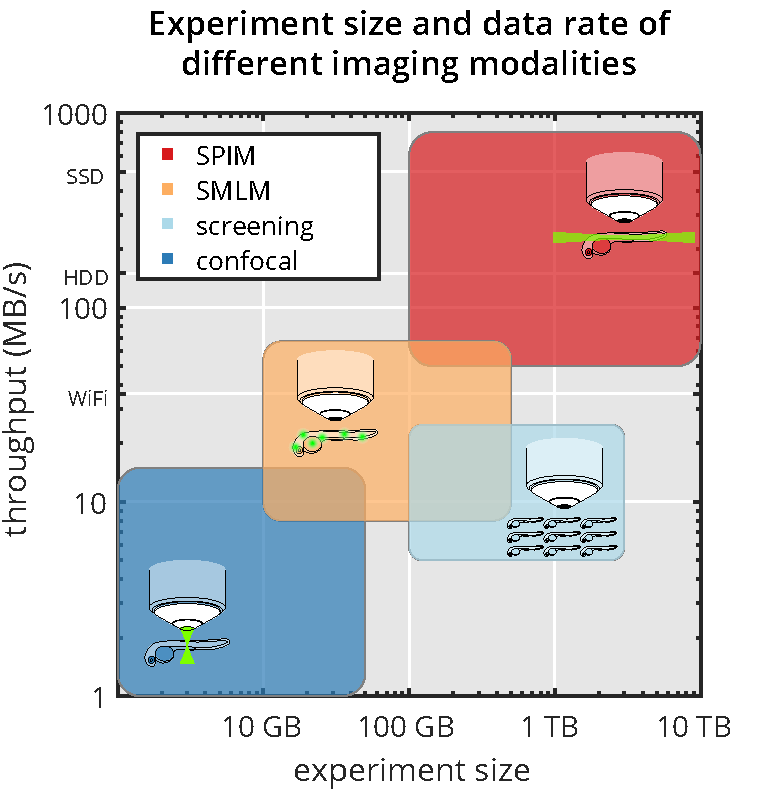
\includegraphics[page=1,width=0.5\textwidth]{comparison_with_pictograms}
    \bcaption[Experiment sizes and data rate of different imaging modalities]{Comparison of single-plane illumination microscopy (SPIM, red), high-content screening (light blue), single molecule localization microscopy (SMLM, orange) and confocal microscopy (blue) by typical experiment size and data production rate (see also \autoref{tab:sizes} in Appendix \ref{app:tables}).}
    \label{fig:sizes}
  \end{figure}

  % To efficiently and quickly process such amounts of information, developing new strategies / innovative approaches is indispensible. As image processing tasks are typically highly parallelizable 

  This chapter will focus on addressing these challenges by presenting a real-time, GPU-based image preprocessing pipeline developed in CUDA \cite{nickolls_scalable_2008} consisting of two parts (\autoref{fig:pipeline}).
  The first part is a fast image fusion method for our workhorse light-sheet microscope, the MuVi-SPIM \cite{krzic_multiview_2012}, that enables live fusion of the images arriving from two opposing cameras.
  The second part of the pipeline, which can also be used in a standalone way, is a real-time image compression library that allows for lossless and noise-dependent lossy compression of the data directly during acquisition even for high-speed sCMOS cameras.

  % To ensure high performance while still keeping the central processing unit (CPU) of the computer available for imaging tasks, we developed our compression algorithm in the CUDA framework \cite{nickolls_scalable_2008} that utilizes the massively parallel architecture of the graphics processing unit (GPU). 

  \begin{figure}
    \centering
    \includegraphics[width=\textwidth]{pipeline}
    \bcaption[Real-time image processing pipeline for multiview light-sheet microscopy]{}
    \label{fig:pipeline}
  \end{figure}



  % \section{CUDA architecture}

  %   CUDA \cite{nickolls_scalable_2008}
  %   CUDA programming Guide \cite{nvidia_cuda_2015}



    % ######## ##     ##  ######  ####  #######  ##    ## 
    % ##       ##     ## ##    ##  ##  ##     ## ###   ## 
    % ##       ##     ## ##        ##  ##     ## ####  ## 
    % ######   ##     ##  ######   ##  ##     ## ## ## ## 
    % ##       ##     ##       ##  ##  ##     ## ##  #### 
    % ##       ##     ## ##    ##  ##  ##     ## ##   ### 
    % ##        #######   ######  ####  #######  ##    ## 

\section{Real-time preprocessing pipeline}

Similarly to the DualMouse-SPIM, our currently used production microscope, the Multiview-SPIM (MuVi-SPIM) \cite{krzic_multiview_2012} also uses multiple imaging directions to improve the image quality. In this case, however, the aim is completeness rather than increasing the resolution. As the MuVi-SPIM is capable of imaging much larger specimens, such as entire \textit{Drosophila} embryos, the sample size itself can present some challenges, especially for opaques specimens. As light scattering and absorption impact both the illumination and detection optics, the negative effects for SPIM are more pronounced compared to single-lens systems \cite{de_medeiros_deep_2016}.




\subsection{Multiview SPIM for \textit{in toto} imaging}

MuVi-SPIM  provides an elegant solution for multiview imaging. A standard SPIM setup with a single detection and a single illumination lens would rotate the sample to acquire images from multiple directions. MuVi-SPIM, on the other hand, utilizes two opposing objectives for illumination and two opposing objectives for detection (\autoref{fig:muvi-spim}a). As the sample is held by an aqueous gel inside the imaging chamber, all objectives have unobstructed view of it from multiple directions (\autoref{fig:muvi-spim}b,c).

Data acquisition is done in two steps: the sample is illuminated by light-sheet 1, and fluorescence is collected by both detection objectives at the same time. After this, light-sheet 2 is activated and both cameras record the fluorescence again (\autoref{fig:muvi-spim}d). This process will result in 4 datasets, all with partial information due to scattering effects. The 4 views are later fused to a single, high quality dataset (\autoref{fig:muvi-spim}e). This fusion process is necessary before any further analysis steps can be performed. However, due to the sheer size of the data, it takes a considerable amount of time after the acquisition.

By combining scanned light-sheet \cite{keller_reconstruction_2008} with confocal slit detection on the camera chip \cite{baumgart_scanned_2012}, it is possible to exclude out-of-focus, scattered illumination light. This way it is  possible to illuminate simultaneously with both light-sheets, which leaves us with only two views, the views of the two opposing cameras \cite{de_medeiros_confocal_2015}.

\begin{figure}
  \centering
  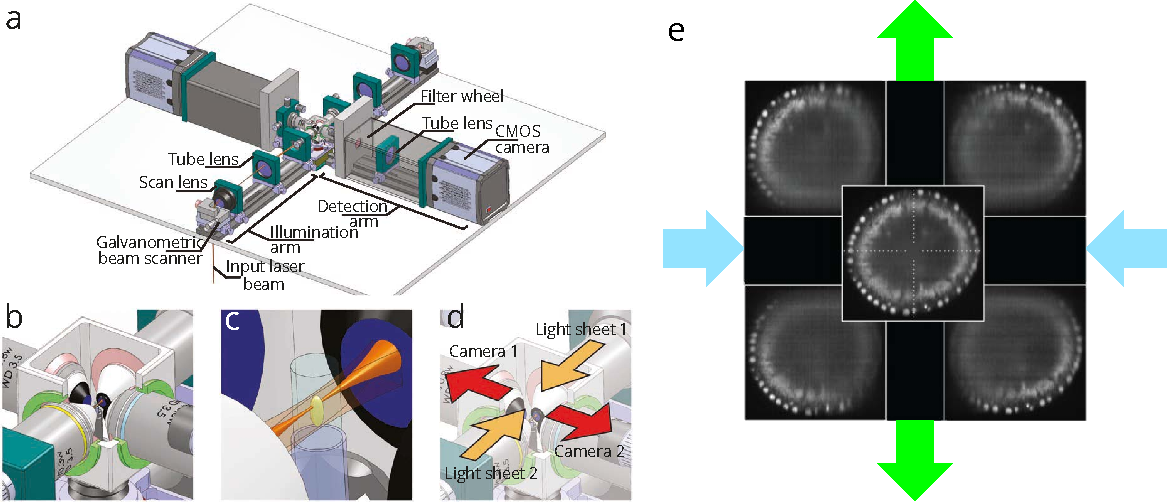
\includegraphics[width=1\columnwidth]{fusion/muvi-spim}
  \bcaption[Operating principle of MuVi-SPIM]{(a) The microscope consists of two illumination and two detection arms for simultaneous multiview illumination and detection. (b) The 4 arms meet in the imaging chamber that is filled with water, and contains the sample. (c) The sample is held by a glass capillary, in  a GelRite cylinder. Optical sectioning is achieved by a virtual light-sheet. (d) The light-sheets can be generated from two sides (light-sheet 1 and 2), and detection is also double sided (Camera 1 and 2). Adapted from \cite{krzic_multiview_2012}.}
  \label{fig:muvi-spim}
\end{figure}




\subsection{Image registration}

To perform image fusion of multiple views, first image registration is necessary: the coordinate systems of the views have to be properly overlapped. Ideally a single mirroring transformation would be enough to superpose the two camera images, however, in practice the microscope can never be aligned with such precision. Other types of transformations are also necessary: translation to account for offsets in the field of view; scaling in case of slightly different magnifications; and also shearing if the detection plane is not perfectly perpendicular to the sample movement direction \cite{krzic_multiple-view_2009}. To combine all of these effects, a full, 3D affine transformation is necessary to properly align the two camera images (\autoref{fig:acquisition} a). This transformation can be represented by a matrix multiplication with 12 different parameters:
\[  
\begin{pmatrix}
x,\\
y,\\
z,\\
1
\end{pmatrix}
=
\begin{pmatrix}
a & b & c & d \\ 
e & f & g & h \\ 
i & j & k & l \\
0 & 0 & 0 & 1 
\end{pmatrix}
\times
\begin{pmatrix}
x\\
y\\
z\\
1
\end{pmatrix}
=
\begin{pmatrix}
a x + b y + c z + d\\ 
e x + f y + g z + h\\ 
i x + j y + k z + l\\
1
\end{pmatrix}
\]
where $x, y, z$ are the coordinates in the original 3D image, $x', y', z'$ are coordinates in the transformed image, and $a, b, ..., l$ are the affine transformation parameters.

These parameters are traditionally acquired by a bead based registration algorithm after imaging fluorescent beads from each view of the microscope \cite{preibisch_bead-based_2009,preibisch_software_2010}. The beads are segmented by using a difference of Gaussian filter, and the registration parameters are acquired by matching the segmented bead coordinates in each view. Identifying the corresponding beads is done by a translation and rotation invariant local geometric descriptor. This matches the beads based on their relative position to their nearest neighbors. After the matching beads are identified, the affine transformation parameters are calculated by minimizing the global displacement for each pair of beads.

For the two opposing views of MuVi-SPIM, these parameters are only dependent on the optical setup itself, and not on the sample or on the experiment. Because of this, it is sufficient to determine the transformation parameters only after modifying the microscope (\textit{e.g.}, after realignment).

In our currently used fusion pipeline, after the parameters are acquired, the 3D stacks are fused by transforming one of the views to the coordinate system of the other (using the affine transformation parameters from the bead based registration), and fusing the two stack by applying a sigmoidal weighted average (\ref{fig:acquisition}a). The weights are determined in a way to exclude the parts of the stacks that have worse image quality and complement these from the other view's high quality regions. When using the electronic confocal slit detection (eCSD) weighting is not necessary, as the scattered light is already rejected in these recordings, and a simple sum of the two stacks gives the best result regardless of the sample \cite{de_medeiros_confocal_2015}.

The fusion process itself can be very resource intensive and can take a considerable amount of time. This is simply due to the size of the 3D stacks: a single dataset is usually between 2 and \SI{4}{GB} in size. Thus, the necessary memory requirement to fuse 2 of these stacks is $3\cdot \SI{4}{GB} = \SI{12}{GB}$, as the result will also take up the same space. Just reading and writing this amount of information to the hard disk takes a substantial amount of time. When using an SSD drive for example, with a \SI{500}{MB/s} read and write speed, just the read/write operations will take around $\frac{\SI{12}{GB}}{\SI{500}{MB/s}} = \SI{24}{s}$.


\begin{figure}
  \centering
  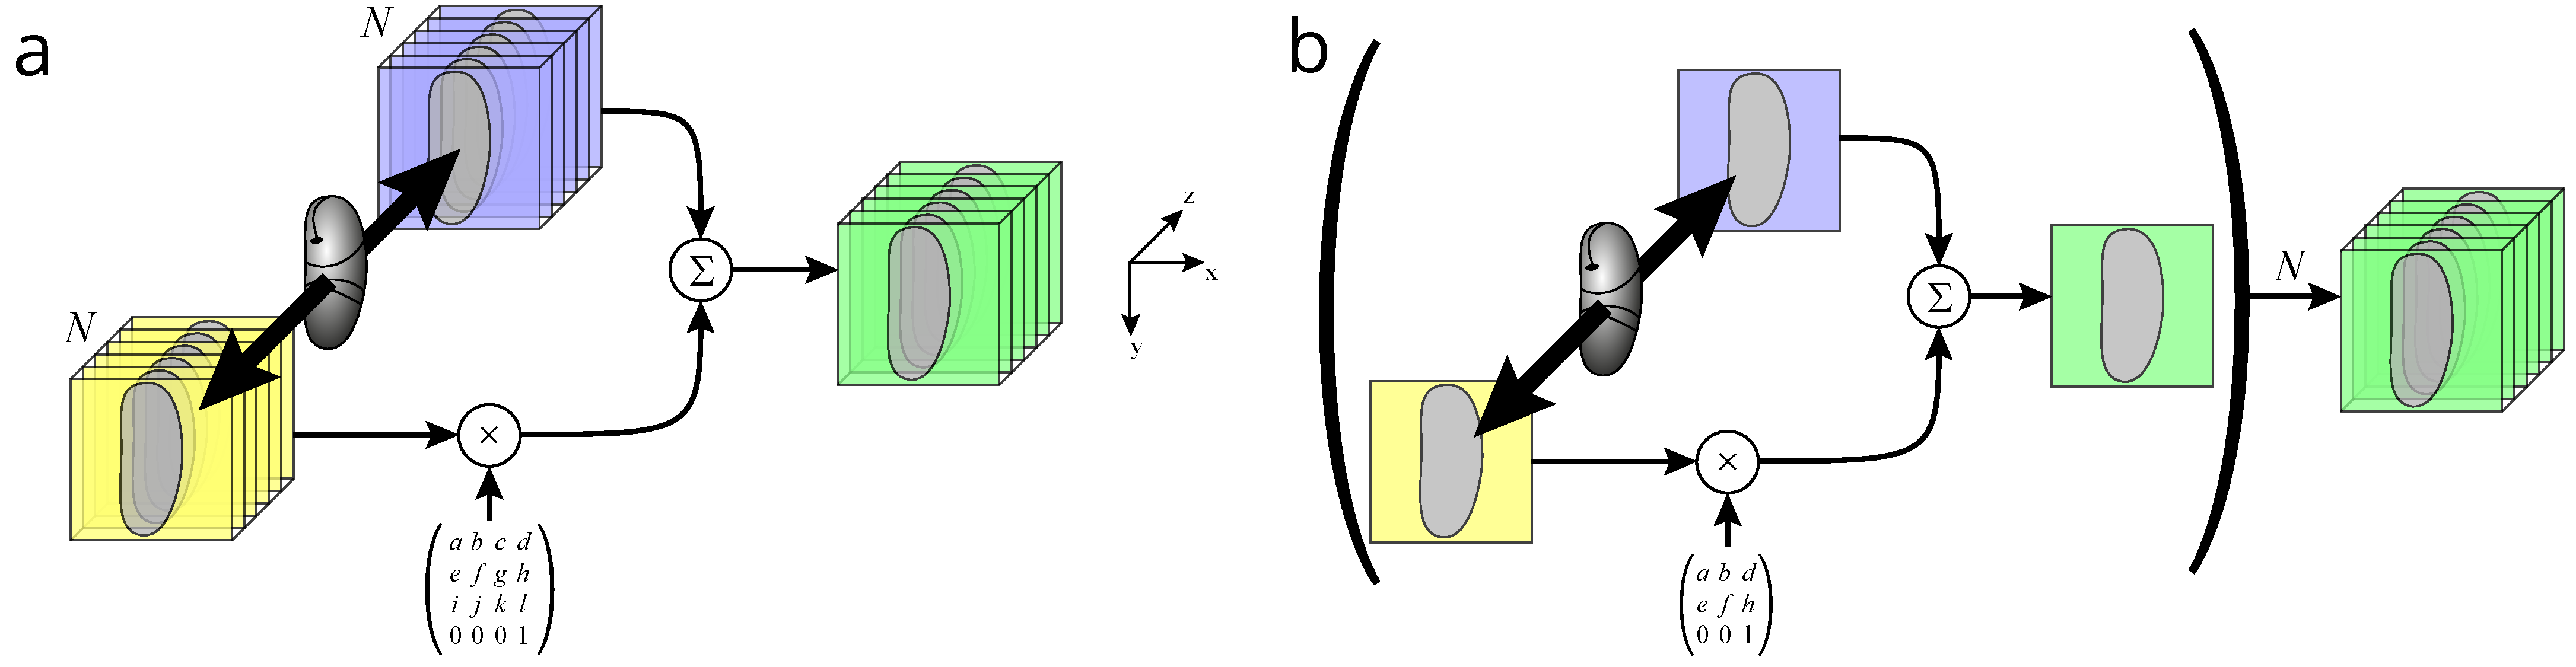
\includegraphics[width=1\columnwidth]{fusion/acquisition}
  \bcaption[multiview fusion methods for light-sheet microscopy]{a) Full 3D stacks are acquired from the opposing views (yellow and blue), which are then registered in 3D space using previously acquired affine transformation parameters. Registered stacks are then weighted averaged to create the final fused stack (green). b) Images from opposing views are directly fused plane by plane. Registration takes place in 2D space thus reducing computational effort and memory requirements. The registered planes are then weighted averaged to create the final fused image.}
  \label{fig:acquisition}
\end{figure}

\subsection{2D fusion of opposing views}
To speed up the image processing, we take a new approach to fusing the images. As the two objectives of MuVi-SPIM ideally image the same $z$ plane, it should be possible to reduce the alignment problem to a 2D affine transformation:
\[ 
\begin{pmatrix}
x'\\
y'\\
1
\end{pmatrix}
=
\begin{pmatrix}
a & b & d\\ 
e & f & h \\
0 & 0 & 1
\end{pmatrix}
\times
\begin{pmatrix}
x\\
y\\
1
\end{pmatrix}
=
\begin{pmatrix}
a x + b y + d\\ 
e x + f y + h\\
1
\end{pmatrix}
\]
The advantage of a simplified transformation is not only the reduced computational complexity, but also the massively reduced memory requirement, as in this case it is sufficient to store 3 planes in memory instead of 3 entire stacks (\autoref{fig:acquisition} b). Performing the 2D direct fusion on the GPU immediately after acquisition has two benefits: first, only the fused images are stored on the hard drive, which directly results in 50\% savings in storage space. Second, since the fusion is faster than the camera acquisition speed, the fused image can be displayed for the users instead of the 2 raw images. This would greatly improve user experience and speed up the initial set-up phase of each experiment.

In order to allow for the direct 2D fusion, the microscope needs to be very well aligned to minimize any adverse effects arising from discarding some of the transformation parameters. The requirements for this are the following:
\begin{align}
\left| c z \right| &< \sigma_{xy} & \forall z \label{eq:req1}\\
\left| g z \right|  &< \sigma_{xy} & \forall z \label{eq:req2}\\
\left| i x + j y + (k-1)  z + l \right| &< \sigma_z & \forall x, y, z  \label{eq:req3}
\end{align}
where $\sigma_{xy}$ is the lateral resolution, and $\sigma_z$ is the axial resolution of the microscope, which are \SI{277}{nm} and \SI{1099}{nm} respectively. 

 If these conditions are fulfilled (\textit{i.e.}, the microscope is properly aligned), direct plane by plane fusion will not result in any loss of information compared to the full 3D image fusion.

% \subsection{Image preprocessing pipeline}

% \begin{figure}[bth]
% \centering
% \includegraphics[width=0.4\columnwidth]{fusion/pipeline}
% \caption{Image preprocessing pipeline. The pipeline comprises of two parts: processing on CPU (white background) and processing on GPU (green background). Images are first transferred from the CPU to the GPU, where the preprocessing steps take place. These include background subtraction, affine transformation, weighted averaging and optionally thumbnail generation and image compression. After the preprocessing steps the image is transferred back to the CPU, and saved on the hard drive, or streamed to a remote computer. Data sizes after each preprocessing step are shown in the gray bands for planes, stacks and time-lapses.}
% \label{fig:pipeline}
% \end{figure}

% To perform the image fusion step as fast as possible, thus enabling it is use for live imaging, we used CUDA (Compute Unified Device Architecture) \cite{_cuda_????-1} to implement the algorithm on a graphics card (NVIDIA, GTX 750). This architecture offers a convenient way to harness the massively parallel computing capabilities of the many streaming multiprocessors residing on a GPU (graphics processing unit). Since each processing step we require is pixel based, they can be inherently parallelized to gain tremendous advantage in computing time.

% To utilize the GPU for the image processing step, the images first have to be transferred from the computer main memory to the graphics card memory. Because of the limited bandwidth of the PCIe 2.0 16x bus, this step is actually the bottleneck, and not the computation itself. To optimize data transfer speed, several techniques can be used.

% First, one has to make sure that the space for the original image data is allocated as paged-lock memory. This is possible with \texttt{cudaMallocHost}. This function will make sure that the memory space allocated on the host will be page-locked, \textit{i.e.}, it is contents cannot be temporarily swapped to the pagefile on the hard disk, and it is actually mapped to the physical memory. Otherwise, with normal allocation functions this is not guaranteed by the operating system, and the memory is only mapped to the physical memory when it is contents are accessed, which heavily influence read/write speed.

% Second, if the same operation is carried out for many images (as in the case of our live fusion method), the data transfer for the next image can already be carried out while the previous image is being processed, thus masking at least one of the data transfers between the main memory and the graphics card.

% % Even when using both methods, most of the time is still taken by the data transfer. Because of this, we decided to implement additional image preprocessing steps in our pipeline (Fig \ref{fig:pipeline}, thus ...

% %To maximize GPU utilization, and ultimately justify the long data transfer times, in addition to the plane by plane fusion (which is actually an affine transformation followed by weighted average), we also implemented background subtraction, subsampling, LUT conversion from 16 bits to 8 bits, and JPEG compression in our pipeline (Fig \ref{fig:pipeline}). All of these steps either enhance image quality (such as background subtraction), reduce data size (LUT conversion, subsampling, JPEG), or both (fusion).


\subsection{CUDA implementation of direct fusion}

  \begin{figure}
    \centering
    \begin{subfigure}[t]{0.49\textwidth}
      \centering
      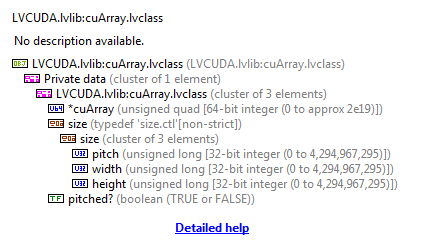
\includegraphics[width=\textwidth]{fusion/CuArray}
      \caption{}
    \end{subfigure}
    \begin{subfigure}[t]{0.49\textwidth}
      \centering
      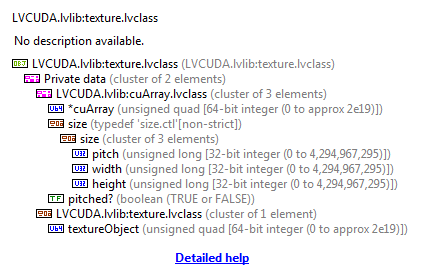
\includegraphics[width=\textwidth]{fusion/Texture}
      \caption{}
    \end{subfigure}
    \bcaption[Classes of LVCUDA library]{(a) \texttt{CuArray} class, wrapping a 1D or 2D pitched device memory for use in LabVIEW. (b) \texttt{Texture} class, wrapping a CUDA texture object for use in LabVIEW.}
    \label{fig:LVCUDA}
  \end{figure}

  Our custom microscope control software (\autoref{sec:software}) is developed in LabVIEW, and we implemented the pipeline as a combination of a CUDA and a LabVIEW library. The CUDA library implements all the necessary low level functions and exposes these in a dynamically linked library (dll). The LabVIEW library, \texttt{LVCUDA.lvlib} implements two high level classes: \texttt{cuArray} and \texttt{Texture} (\autoref{fig:LVCUDA}). These classes interface with the CUDA dll, and allow to easily build a flexible CUDA-based image processing pipeline in LabVIEW.

  As the pipeline operates on 2D images, both classes support 1D or 2D arrays in a pitched configuration. \texttt{CuArray}, as the parent class, stores the pointer to the array, as well as the pitch, width and height. LabVIEW natively doesn't support pointer operations, therefore the pointer is simply cast to a \SI{64}{bit} unsigned integer internally. As this is a private member of the class there is no danger of accidental modification. Being a descendent of \texttt{cuArray} class, the \texttt{Texture} class adds a further member to store the reference to the CUDA texture object. This class is used to implement the affine transformation, as it supports floating point indexing and automatic linear interpolation.

  Since the processing is actually bottlenecked by the data transfer rate between the main memory and GPU memory, we implemented multiple commonly used image preprocessing operations for our pipeline to maximize the utility of the GPU. These functions include background subtraction, background masking and image compression. We will discuss these features in the following sections of the chapter. 


  \subsection{Background subtraction and masking}
  
  \begin{figure}
    \centering
    \begin{subfigure}{0.49\textwidth}
      \centering
      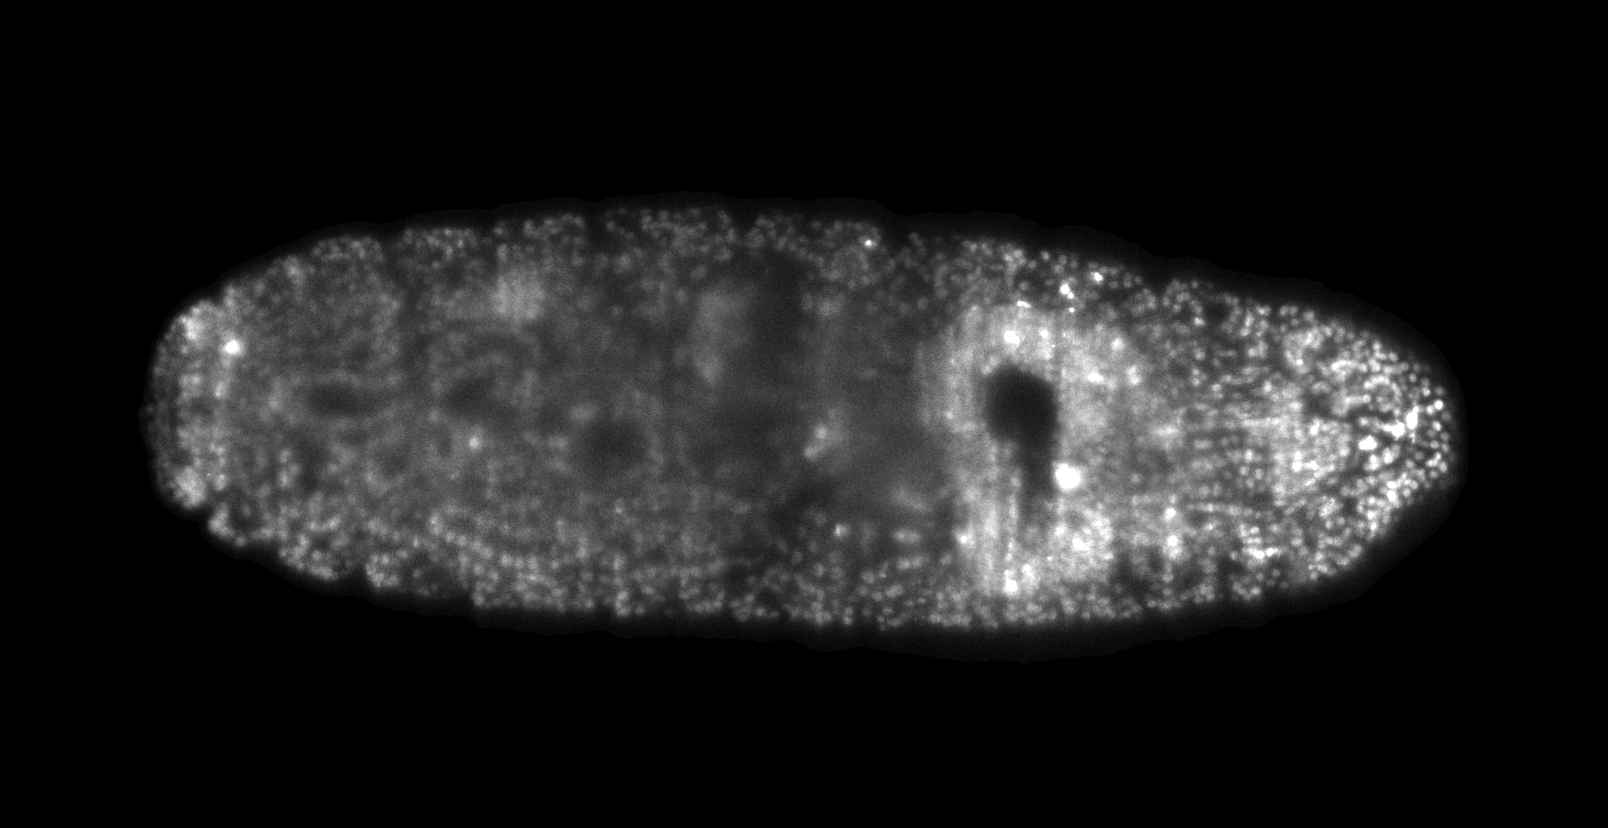
\includegraphics[width=\textwidth]{fusion/drosophila_not_masked}
      \caption{}
    \end{subfigure}
    \begin{subfigure}{0.49\textwidth}
      \centering
      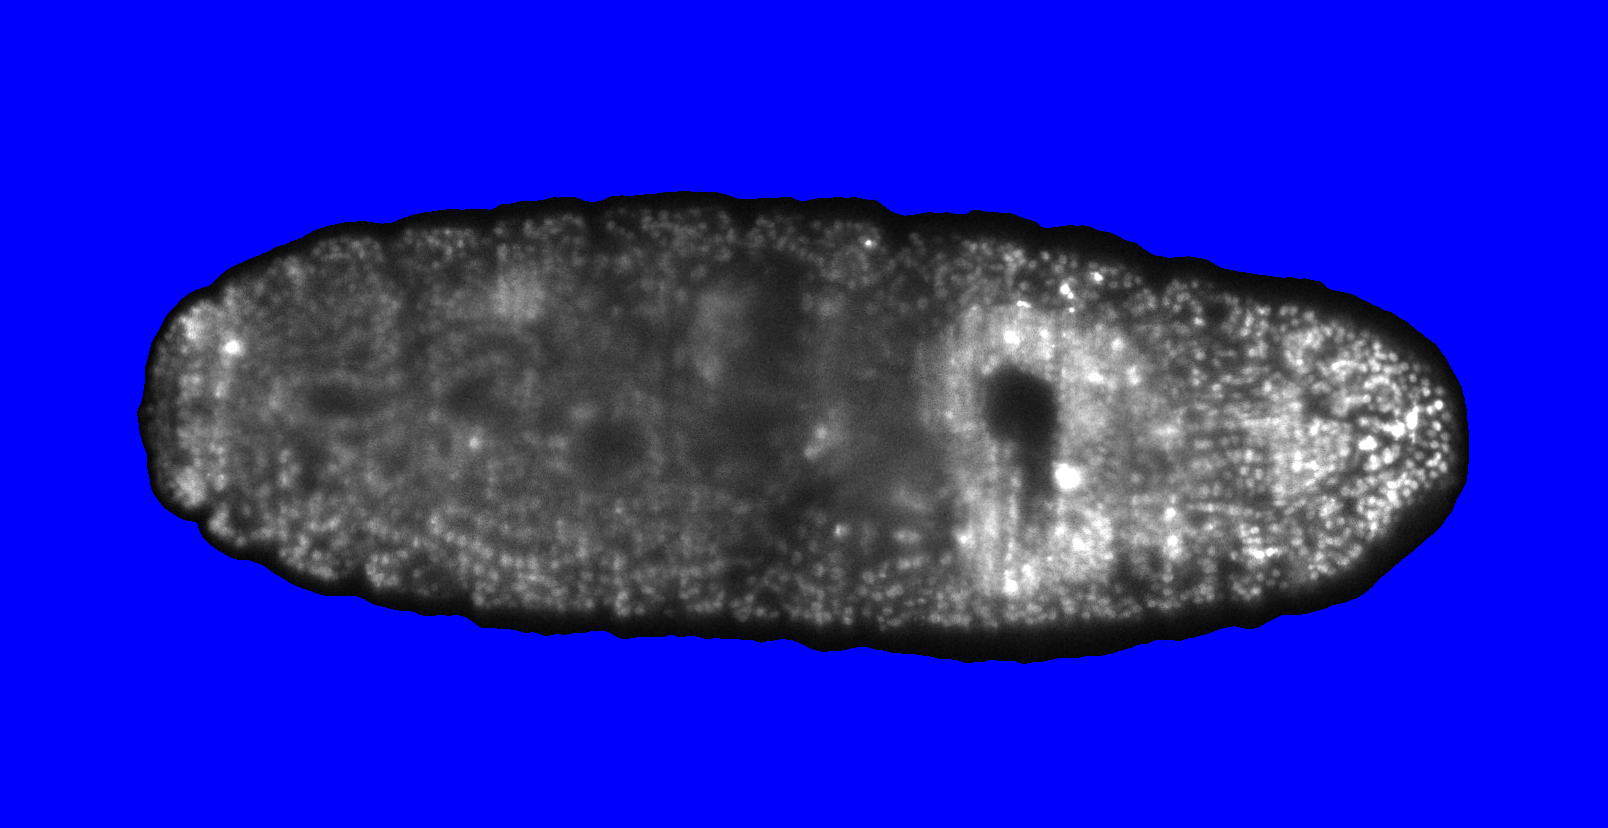
\includegraphics[width=\textwidth]{fusion/drosophila_masked}
      \caption{}
    \end{subfigure}
    \bcaption[Applying mask to remove background]{(a) Original image of a \textit{Drosophila} embryo. (b) Background selected by thresholding the blurred image.}
    \label{fig:masking}
  \end{figure}
  
  As an additional step of the preprocessing pipeline, background subtraction and background masking was implemented. Background subtraction can improve image quality as it removes any system-specific patterns, while background masking is beneficial for the consecutive compression step.

  To perform the background subtraction, dark images are recorded without the laser turned on. Typically 500--2000 images are taken which are averaged, to capture the pixel non-uniformities of the camera sensors. As this is camera specific, the step is repeated for all cameras. If necessary, the recordings can be repeated under different conditions, such as different exposure times, or different sensor modes (such as global shutter and rolling shutter). The averaged background images are saved in a custom file format in an HDF5 container \cite{the_hdf_group_hierarchical_1997} together with the camera serial number. The microscope software can read these files and applies the background subtraction to the appropriate cameras during imaging.

  Background masking is a useful step to increase the efficiency of image compression. For light-sheet microscopy, where typically an entire embryo is imaged, the boundary of the specimen, and thus the area of interest, is well defined. Anything outside the embryo is just noise which does not contribute to any useful information. For image compression, however, these regions are extremely difficult to compress, as due to the random nature of noise, almost no reduction is achievable (see \ref{sec:entropy}). To circumvent this issue, the background pixels outside the specimen can be set to 0, which will greatly increase the compression ratio without compromising any data of interest \cite{amat_efficient_2015}.

  The masking is performed in the following way. As the sample has much higher signal compared to the background, a thresholding operation is sufficient. In order to have a smooth mask, the images are first blurred by a Gaussian kernel, and the thresholding is done on the blurred image. This will define a binary mask with smooth boundaries, which is applied to the original image (\autoref{fig:masking}). The threshold can be calculated automatically by the Triangle method \cite{zack_automatic_1977}, or can also be user specified.

  

  


\subsection{Methods and results}


\begin{figure}
  \centering
  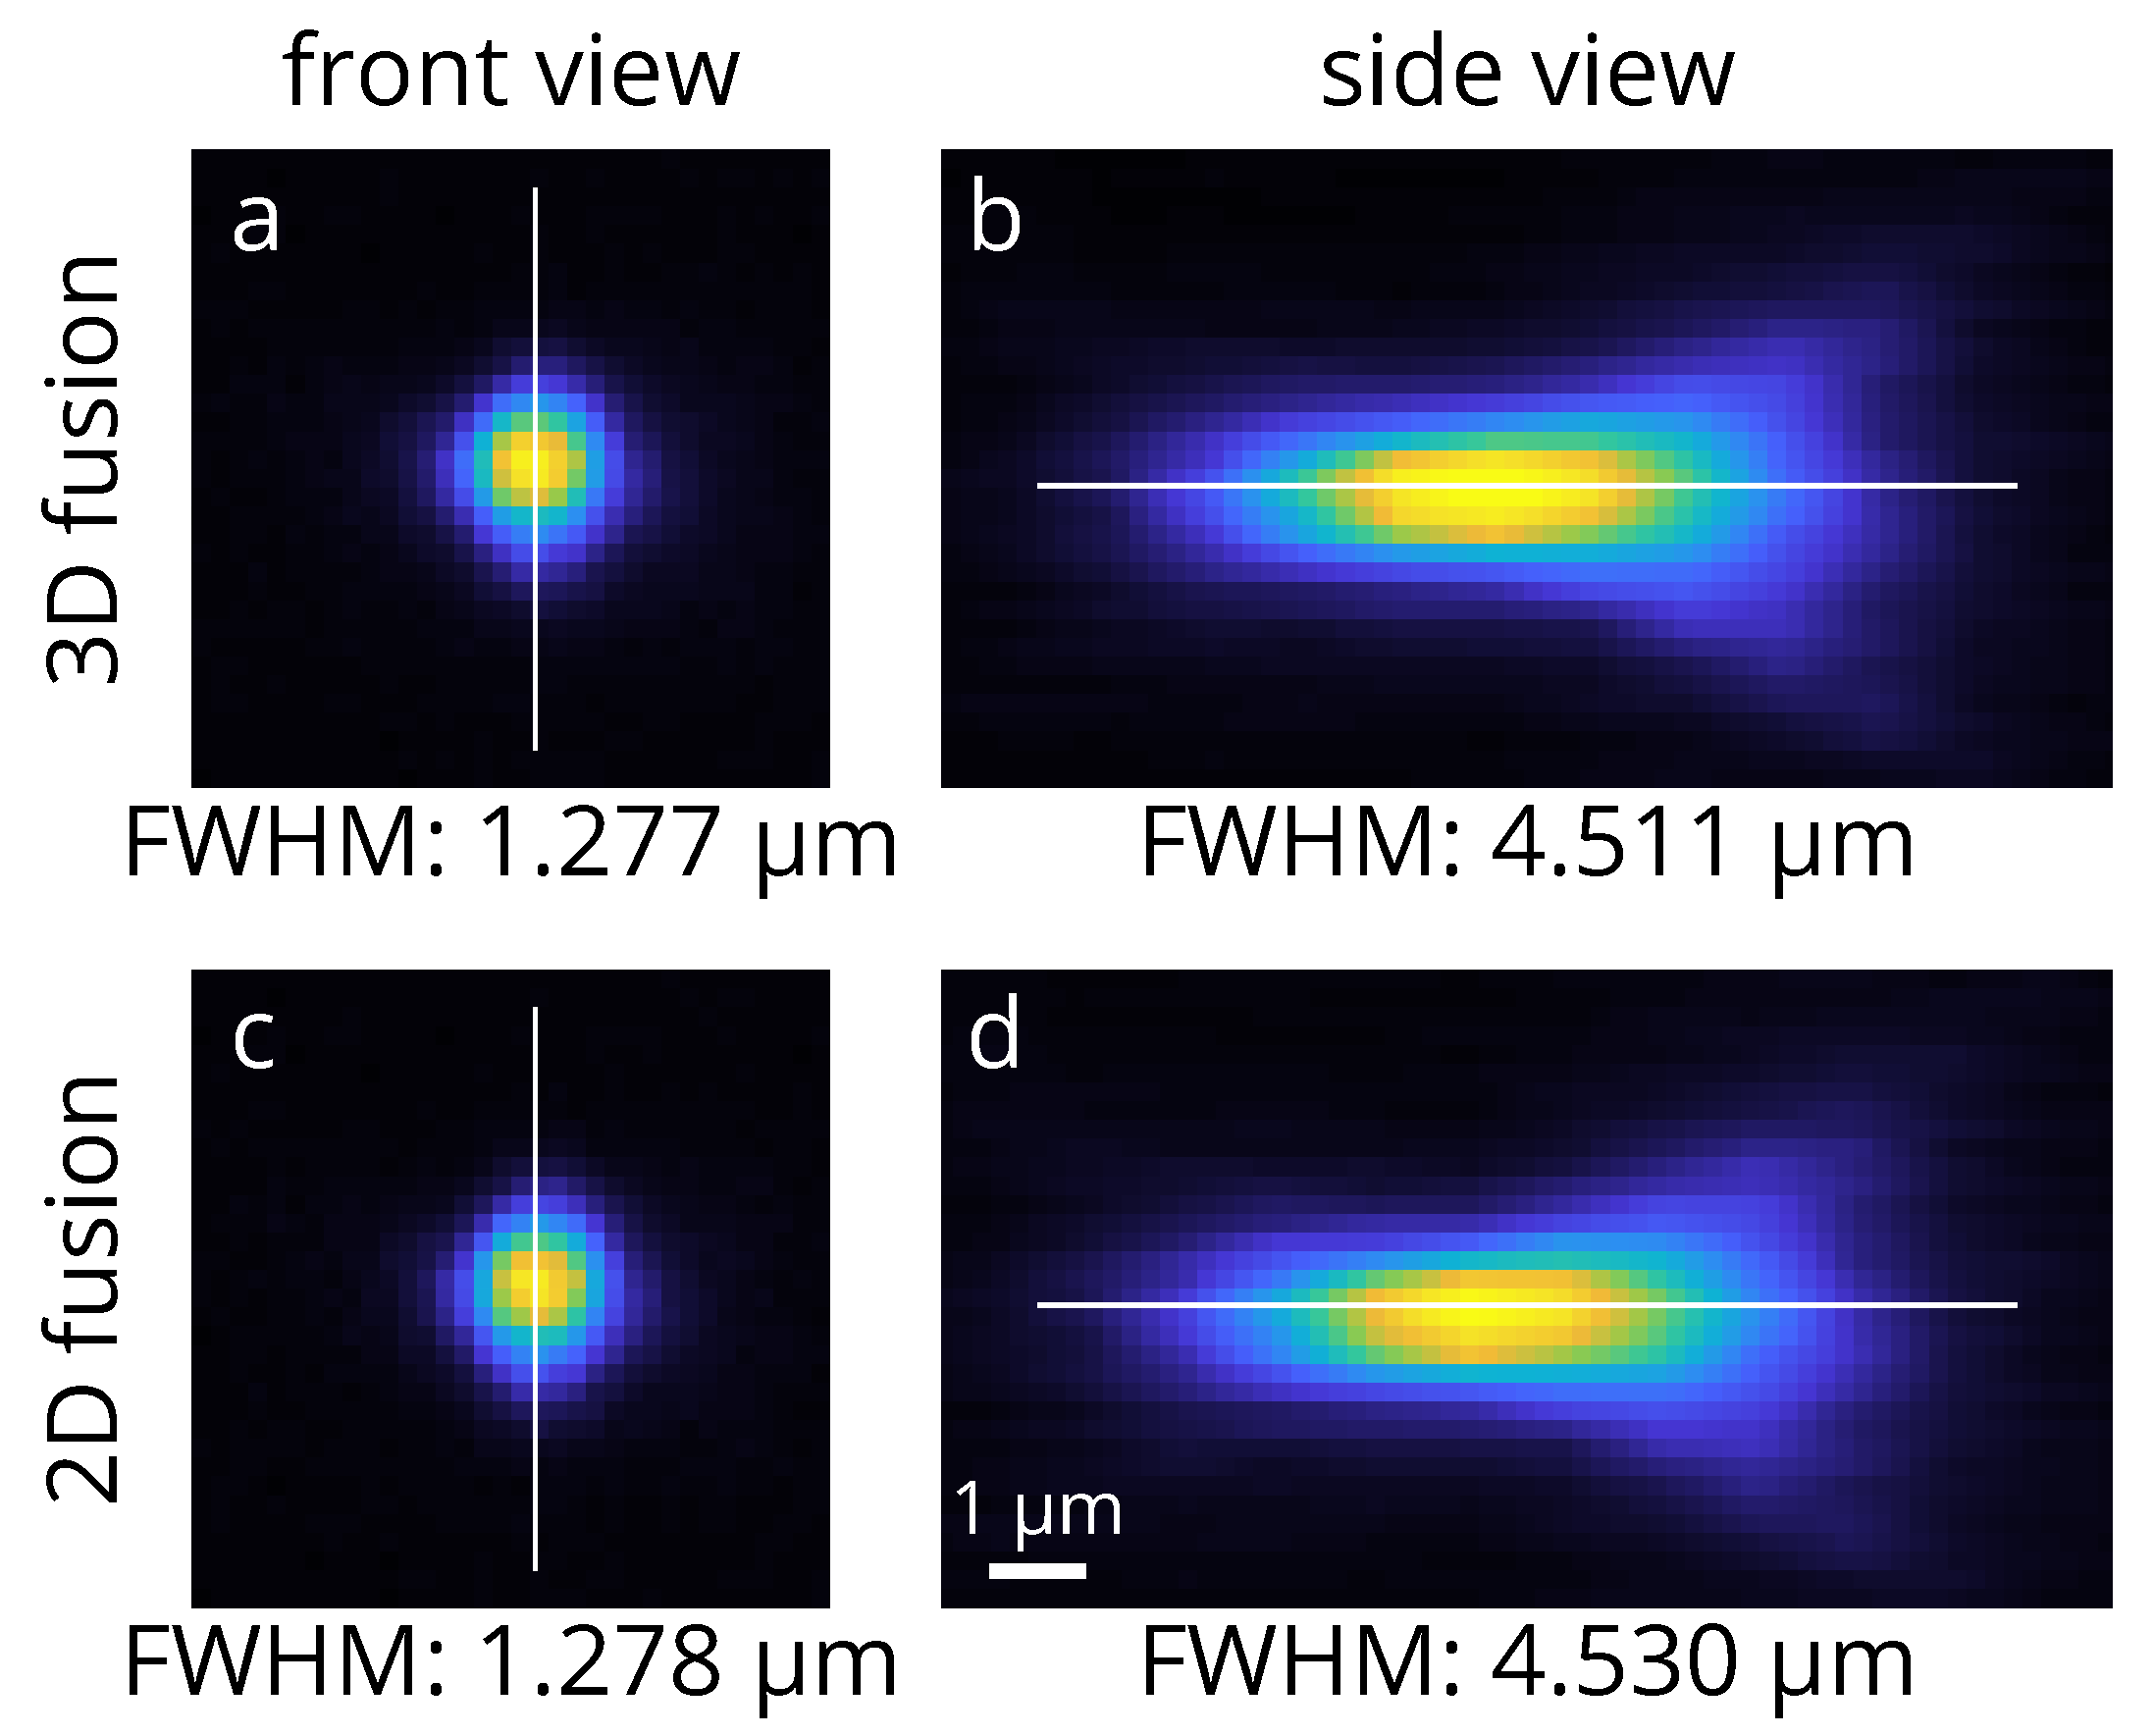
\includegraphics[width=0.6\textwidth]{fusion/beads/2Dvs3Dbeads}
  \bcaption[Comparison of 3D and 2D fusion of beads]{Front and side views of a representative bead after 3D full affine fusion (a, b) and after 2D planewise fusion (c,d). FHWM was measured along the indicated lines, through the center of the bead image. Scale bar: \SI{1}{\micro m}.}
  \label{fig:2Dvs3Dbeads}
\end{figure}

  The image preprocessing pipeline was tested on our MuVi-SPIM microscope \cite{krzic_multiview_2012}.   
  Processing speed of the CPU and GPU implementation of the processing pipeline was measured with the profiling tool of LabVIEW, and are an average of 10 runs. The benchmarking computer had 2 Intel Xeon E5620 processors with 8 processing cores running at \SI{2.4}{GHz}, \SI{24}{GB} RAM and an Nvidia GeForce GTX 750 graphics card. Test images were 2048\texttimes 2048 pixels at \SI{16}{bit} depth. 
  
  For the background subtraction we recorded 1500 dark images with each camera and averaged them, in order to obtain the camera specific background images. Prior to image acquisition these were uploaded to the GPU memory, and were readily available for the pipeline. The implemented CUDA pipeline with background subtraction, 2D fusion and masking reached a throughput of 135.8 frames per second (fps), while a single-threaded CPU implementation could only process 7.4 images per second on average.

  

  Following careful alignment of the microscope to meet the previously discussed requirements (Eqs. \ref{eq:req1} -- \ref{eq:req3}), we imaged fluorescent beads in a gel suspension to obtain the affine transformation parameters. The measured 3D transformation parameters were the following:

  \[
  \begin{pmatrix}
    1.013 & 2.494\times 10^{-3} & \mathbf{7.182\times 10^{-3}} & -21.67 \\
    -1.697\times 10^{-3} & 1.014 & \mathbf{-3.192\times 10^{-5}} & -4.161 \\
    \mathbf{-9.694\times 10^{-5}} & \mathbf{1.937\times 10^{-7}} & \mathbf{1.003} & \mathbf{-0.433} \\
    0 & 0 & 0 & 1
  \end{pmatrix}
  \]
  Substituting these values to Eqs. \ref{eq:req1} -- \ref{eq:req3} and evaluating for the full range of $x, y, z$, the maximum contribution of the discarded coefficients for each coordinate will be:
  \begin{align*}
    \max |cz| =& \SI{0.070}{\micro m}  \\
    \max |gz| =& \SI{3.11e-4}{\micro m}  \\
    \max | i x + j y + (k-1)  z + l | =& \SI{0.7789}{\micro m}
  \end{align*}
  As these are below the resolution of the microscope, discarding the coefficients and reducing the 3D transformation to a 2D transformation will not have any negative effects on the image quality.
  % x, y 0..2048, z -50..50

  

  To validate our hypotheses, we fused bead stacks that were acquired for the calibration using both the 3D and the 2D transformations. The 2D, planewise fused beads do not exhibit any pathological morphologies compared to the 3D fused beads (\autoref{fig:2Dvs3Dbeads}). When measuring the size of the bead images (FWHM) along the lateral and axial directions, the difference is less than 0.5\% compared to the 3D fused dataset. This is well below any resolvable features.

  \begin{figure}
    \centering
    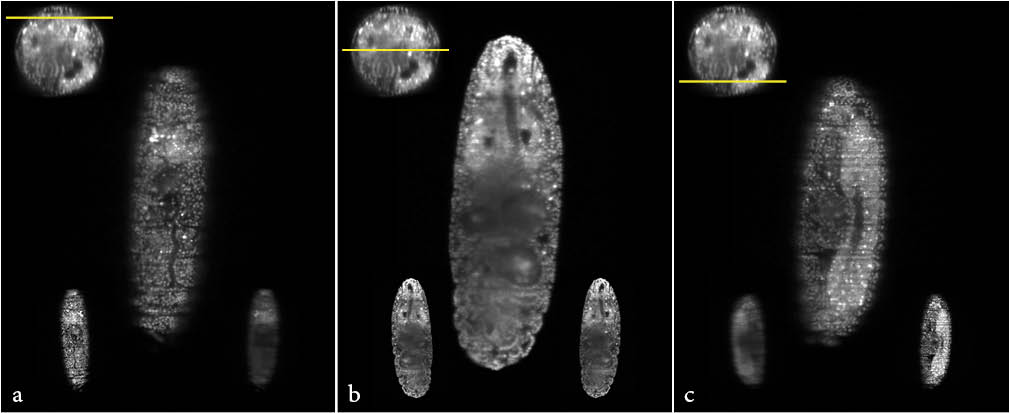
\includegraphics[width=1\textwidth]{fusion/drosophila_D2}
    \bcaption[GPU fused images of a \textit{Drosophila melanogaster} embryo]{Two stacks were taken in quick succession first without fusion, then with fusion enabled. Fused images are shown in the middle of each subfigure, while the individual camera images are in the bottom insets. The top-left inset depicts the z-position of the shown images. (a) Image from closer to the left camera. (b) Image from the center of the embryo. (c) Image from closer to the right camera.}
    \label{fig:drosophila_D2}
  \end{figure}

  \begin{figure}
    \centering
    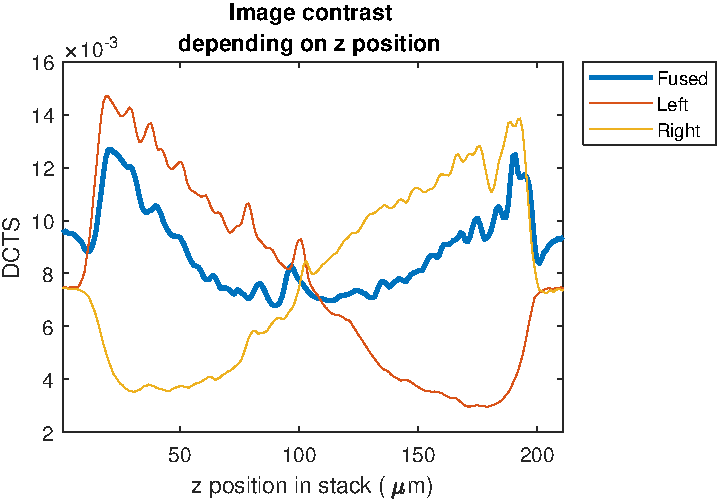
\includegraphics[width=0.7\textwidth]{fusion/drosophilaContrast}
    \bcaption[Image contrast depending on z position for raw and fused stacks]{Image contrast was measured as the Shannon entropy of the normalized Discrete Cosine Transform of the sections \cite{royer_adaptive_2016}. Contrast measurments were performed on the images shown on \autoref{fig:drosophila_D2}.}
    \label{fig:drosophilaContrast}
  \end{figure}

  We applied the direct fusion method to various biological specimens, such as \textit{Drosophila melanogaster} embryos, zebrafish larvae, \textit{Phallusia mammillata} embryo and \textit{Volvox} algae. As a demonstration, here we show the results of imaging a \textit{Drosophila} embryos expressing H2Av-mCherry histone marker. The embryos were imaged first without direct fusion enabled, and immediately afterwards with direct fusion enabled (\autoref{fig:drosophila_D2}). Image quality dependency on the depth of the imaging plane is especially apparent in single-view stacks. Planes closer to the objective give a sharp, high contrast image, while planes deeper inside the embryo are severely degraded due to scattering (\autoref{fig:drosophilaContrast}).

  Stacks obtained with the live fusion enabled show a consistently high image quality throughout the entire stack, independent of the depth (\autoref{fig:drosophilaContrast}). This allows us to keep only the already fused data, thus effectively reducing the storage requirement by half, and facilitating further data processing steps.

  %\subsection{Methods}

 

  


% \section{Conclusions}

% I developed a direct plane by plane fusion method which was implemented in CUDA, and can be performed live, directly on the microscope. This results in a single, high quality recording, which can be directly used later for further processing or data evaluation. We showed the viability of the method by imaging fluorescent beads, and fluorescently labeled \textit{Drosophila m.} embryos, which showed superior image quality to both of the original views. As a further consequence, data handling became easier, less storage is needed for further experiments, and considerable time is spared by eliminating the need for the 3D fusion step.

% For several samples orthogonal views are desired, or in some cases the optical setup is already designed with orthogonal detection\cite{wu_spatially_2013}, or close to orthogonal in the case of the symmetric mouse SPIM. In these cases to properly fuse the different directions, multiview deconvolution is necessary \cite{krzic_multiple-view_2009,temerinac-ott_multiview_2012} to gain maximum information from both views.






%#######   #######  ########  
%#     ## ##     ## ##     ## 
%#     ##        ## ##     ## 
%#######   #######  ##     ## 
%#     ##        ## ##     ## 
%#     ## ##     ## ##     ## 
%#######   #######  ########  
  
\section{\b3d image compression}

  The second part of our GPU-based image preprocessing pipeline is a new image compression algorithm that allows for extremely fast image compression to efficiently reduce data sizes already during acquisition.
  % A straightforward solution to these problems would be to compress the images during acquisition.
  Although this would not reduce the requirements for image processing power and time, it still has a big impact on the necessary background infrastructure. By reducing the data size, not only the cost for storage can be reduced, but also the time it takes to transfer the data during the various steps of data processing is shortened. A fast compression method would also greatly improve 3D data browsing possibilities, as more data could be piped to the rendering software.

  Despite the advantages, real-time compression for high-speed microscopy has not been available, and this is mostly due to the lack of appropriate compression methods suitable for scientific imaging that also offers the high throughput demanded by these applications. While typically used lossless compression methods, such as JPEG2000 \cite{adams_jpeg-2000_2001} offer good compression ratios, they are very slow in processing speed, at least compared to the data rate of a modern microscope ($\sim \SI{1}{GB/s}$, \autoref{fig:sizes}). High-speed compression methods that can deal with this data rate have been developed for ultra-high-definition 4K and 8K digital cameras, such as the high efficiency video codec (HEVC) \cite{international_telecommunications_union_h.265_2016}. These methods, however, have been optimized for lossy image compression which is generally not acceptable for scientific data \cite{cromey_digital_2013}, and rarely support compression of high bit rate originals, which is typically the case for modern sCMOS sensors. Although the HEVC recommendation does specify bit rates up to 16 bits, and lossless compression, the open source version, x265 only supports bit rates up to \SI{12}{bit} \cite{noauthor_x265_nodate}.

  To address these issues, we developed \b3d, a GPU based image compression library capable of high-speed compression of microscopy images during the image acquisition process. By utilizing the massively parallel processing architecture of a GPU, we were not only able to reach a compression and decompression speed of \SI{1}{GB/s}, but our algorithm also keeps the load off the CPU, making it available for other computing tasks related to operating the microscope itself.

  A second feature of our compression library is a novel algorithm for noise-dependent lossy compression of scientific images. Although most lossy compression methods are not suitable for scientific data, our method allows for a deterministic way to control the exact amount of loss. The algorithm was designed in a way that any modification to a single pixel is proportional to the inherent image noise accounting for shot noise and camera read noise. Since this noise already introduces some uncertainty to the raw data, if any changes made are smaller than this, the extractable information by further data analysis steps should be not affected, whereas the compression ratio is massively increased. 
  
  % As mentioned before, lossy compression is not recommended for scientific images, and the reason for this is that practical lossy compression algorithms are designed with the intent of fooling the human visual system \cite{sayood_introduction_2012}. While the images compressed by these algorithms may appear identical to the eye, any downstream data analysis could be negatively impacted by the compression artifacts. To our knowledge, only a single algorithm allows to set the loss in a deterministic manner: the near-lossless operating mode of JPEG-LS \cite{weinberger_loco-i_2000}. In this mode it is possible to set the maximum allowable error a pixel can have after decompression. Although this can be useful for certain applications, it has not been widely implemented, as the visual quality loss is more severe compared to other algorithms with the same compression ratio \cite{santa-cruz_study_2000}.



  % \b3d image compression
  % light-sheet (Sec. \ref{sec:light-sheet})
  % data handling is bottleneck 

  % KLB \cite{amat_efficient_2015}

  % big data viewer \cite{pietzsch_bigdataviewer:_2015}
  % Fiji \cite{schindelin_fiji:_2012}

  % FLIC \cite{wang_fast_2012}
  % SFALIC \cite{starosolski_simple_2007}
  % FELICS \cite{howard_fast_1993} -> this was before JPEG-LS
  % Treib terrain editing \cite{treib_interactive_2012}
  % Treib turbulence \cite{treib_turbulence_2012}



    


    

  \subsection{Compression algorithm}

    % compression scheme: modeling+ coding \cite{rissanen_universal_1981}

    
    \subsubsection{Lossless compression}
    % To ensure high performance while still keeping the central processing unit (CPU) of the computer available for imaging tasks, we developed our compression algorithm in the CUDA framework \cite{nickolls_scalable_2008} that utilizes the massively parallel architecture of the graphics processing unit (GPU). 
    The algorithm design initially had three main requirements to ensure suitability for a high-speed microscopy environment: 1) low complexity for fast execution, 2) no data dependencies to enable parallel execution, and 3) full reversibility to ensure lossless compression. Since existing image compression standards such as JPEG2000 \cite{adams_jpeg-2000_2001} or JPEG-LS \cite{weinberger_loco-i_2000} were designed to maximize compression ratio even at the expense of compression speed, these were not suitable for our needs. Furthermore, most steps inherently require sequential execution, thus preventing efficient parallelization. Promising efforts have been made to enable parallel compression by simplifying JPEG-LS and removing the limiting steps from the algorithm (such as Golomb parameter adaptation or context modeling) \cite{wang_fast_2012,starosolski_simple_2007}. Although some of these methods could reach a significant speedup with minimal expense in compression ratio, their performance was still not enough for real-time compression of high-speed microscopy data.

    As in the case of other image compression methods, our algorithm has two main components: decorrelation and entropy coding (\autoref{fig:algorithm}a). In this work we focused on implementing a parallel encoder and decoder for the decorrelation part that would also be compatible with the noise-dependent lossy compression, as efficient CUDA-based entropy coders are already available \cite{treib_interactive_2012}. To decorrelate the data, similarly to JPEG-LS and lossless-JPEG \cite{pennebaker_jpeg:_1992}, a prediction is performed for each pixel by calculating the average of the top and left neighbors (\autoref{fig:algorithm}b). The prediction is subtracted from the real pixel value, resulting in the prediction error term:
    \begin{equation}
      \varepsilon = X - \pred(X).
    \end{equation}
    Since the neighboring pixels have a high chance of correlation, these error terms will typically be very small compared to the raw intensity values. This step is similar to predictor 7 of lossless JPEG (see \ref{sec:predictors}).

    The pixel prediction method is especially well suited for parallel compression, as it can be performed independently for all pixels. For decompression, the top and left neighbor of a pixel need so be first reconstructed, thus parallelization needs some adjustments. An obvious choice is to perform the reverse prediction in tiles, where the number of threads will equal the number of tiles. Parallel execution can be further scaled up if the decoding is done in diagonals, starting from the top left corner (\autoref{fig:algorithm}c). With this method the average number of parallel threads will be
    \begin{equation}
      N_{th} = N_t * a_t / 2,
      \label{eq:numThreads}
    \end{equation}
    where $N_{th}$ is the number of threads, $N_t$ is the number of tiles, $a_t$ is the tile width and height for a square tile. Although the threads can be maximized by making smaller tiles, the compression ratio will be negatively affected. This is because the corner pixel can't be predicted, and for the edges only one neighbor can be used instead of 2. We find square tiles between 16 and 64 pixels are a good choice between decompression speed and compression ratio.
    
    The prediction error terms are subsequently run-length encoded and entropy coded by a fast, CUDA-enabled Huffman coder \cite{treib_interactive_2012,treib_turbulence_2012} to effectively reduce data size. The library is making extensive use of parallel prefix sum, which can be used for the effective parallel execution for both run-length encoding and Huffman coding. For decompression, the Huffman coding and run-length encoding are first reversed, then each pixel value is reconstructed from the neighboring values and the prediction errors. Although this implementation sacrifices a little in compression ratio compared to size-optimized methods, it can surpass a compression speed of \SI{1}{GB/s} (see \autoref{sec:evalB3D}), which is sufficient even for the dual camera confocal MuVi-SPIM setup \cite{de_medeiros_confocal_2015}.
    
    \begin{figure}[tpb]
      \centering
      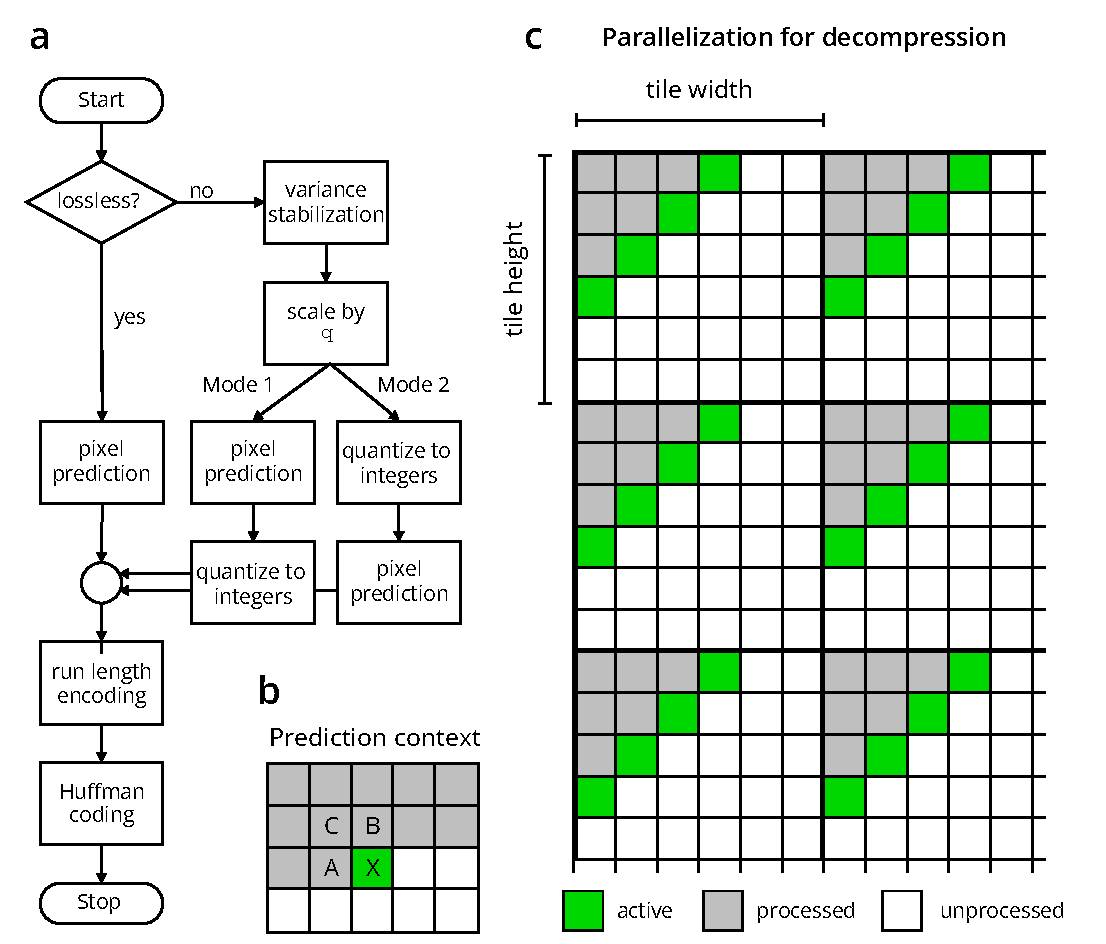
\includegraphics[page=1,width=0.6\textwidth]{tiles}
      \bcaption[\b3d algorithm schematics]{
      
      % (\textbf{b}) Lossless JPEG predictors for X, based on the context showed in (\textbf{a}). The first three predictors are one-dimensional, while the rest are two-dimensional. Using a two dimensional predictor while increases complexity slightly, also increases the achievable compression ratio. We found that for fluorescence microscopy images predictor 7 performs best, hence its inclusion in the \b3d algorithm.
      (\textbf{a)} Complete algorithm flowchart depicting the main stages of the compression.
      % First, if the result should be lossless, pixel prediction is performed on the original image values. If within-noise-level mode is selected, the image noise is stabilized first (see \autoref{sec:wnl}), which is then scaled by the quantization step $q$. Prediction is performed, and the prediction errors are rounded to the nearest integer. The prediction errors for both lossless and lossy modes are then run-length encoded, and finally Huffman coding is applied to effectively reduce data size. The output of the Huffman coder is saved as the compressed file.
      (\textbf{b}) Prediction context for pixel X, the next sample to be encoded. Three neighboring pixels are considered: left (A), top (B) and top left (C) neighbors.
      (\textbf{c}) Parallelization scheme for decompression and lossy compression. Already processed pixels are in gray, unprocessed pixels are in white, active pixels are in green.
      % Since the prediction depends on the top and left neighbors, all green pixels can be calculated independently, in a parallel manner. To increase parallelism, the image is processed in independent tiles.
      }
      \label{fig:algorithm}
    \end{figure}

    \subsubsection{Within-noise-level compression}
    \label{sec:wnl}
    Noise-dependent lossy compression relies on the fact that microscopy images naturally contain photon shot noise. To increase compression ratio, this algorithm allows some differences in the pixel values, as long as they are within a predefined proportion of the inherent noise. A special case for this mode is when all compression errors are smaller than the standard deviation of the noise ($\sigma$), which we call within-noise-level (WNL) compression.

    Our algorithm is inspired by both the near-lossless mode of JPEG-LS \cite{weinberger_loco-i_2000}, where the maximum compression error can be set to a predefined value, and the square root compression scheme \cite{gowen_square_2003, bernstein_noise_2010}, that quantizes its input relative to its square. We combine the two methods to achieve noise-dependent lossy compression while still retaining good image quality and avoiding banding artifacts.

    Before the prediction errors are sent to the entropy coder, a quantization can take place that reduces the number of symbols that need to be encoded in order to increase compression ratio. By changing the quantization step, the maximum absolute reconstruction error can be defined, such as when using JPEG-LS. For noise dependent compression, however, the quantization step should be proportional to the image noise, which can be achieved by the following variance stabilizing transformation introduced by Bernstein \etal \cite{bernstein_noise_2010}:
    \begin{equation}
      T = 2 \sqrt{e + \sigma^2_{RN}},
      \label{eq:wnl}
    \end{equation}    
    where $e$ is the intensity scaled to photoelectrons, and $\sigma_{RN}$ is the standard deviation of the camera read noise. To perform the scaling of digital numbers (DN) to photoelectrons, it’s necessary to know the camera offset and conversion parameters: $e=(I-offset)\cdot g$, where $g$ is the gain in photoelectrons/DN, and $I$ is the original pixel intensity. The transformation assumes a Poisson-Gaussian noise, incorporating the photon shot noise and the camera readout noise, which is a good model for most scientific imaging sensors, such as (EM)CCD or sCMOS.

    To accommodate for all imaging needs, two options are available in the noise-dependent lossy mode. In Mode 1, after the stabilizing transform (\autoref{eq:wnl}), the prediction is performed first, followed by quantization of the prediction errors. This mode reaches a better compression ratio and higher peak signal-to-noise ratio (PSNR) for the same quantization step compared to Mode 2 (\autoref{fig:swapping} a, b), and is recommended for most use cases. For larger quantization steps ($q \geq 3 \sigma$), however, Mode 1 might introduce some spatial correlations, because the prediction errors that are being quantized depend on multiple adjacent pixels (\autoref{fig:swapping} c, d). Mode 2 excludes this possibility by swapping the quantization and prediction (\autoref{fig:swapping} c, d) at the expense of compression ratio. Since no correlations are introduced, Mode 2 is suitable for highly sensitive image analysis tasks, such as single-molecule localization. In this chapter we use Mode 2 for single-molecule localization data, and Mode 1 for all other datasets.
  
    \begin{figure}[bhtp]
      \centering
      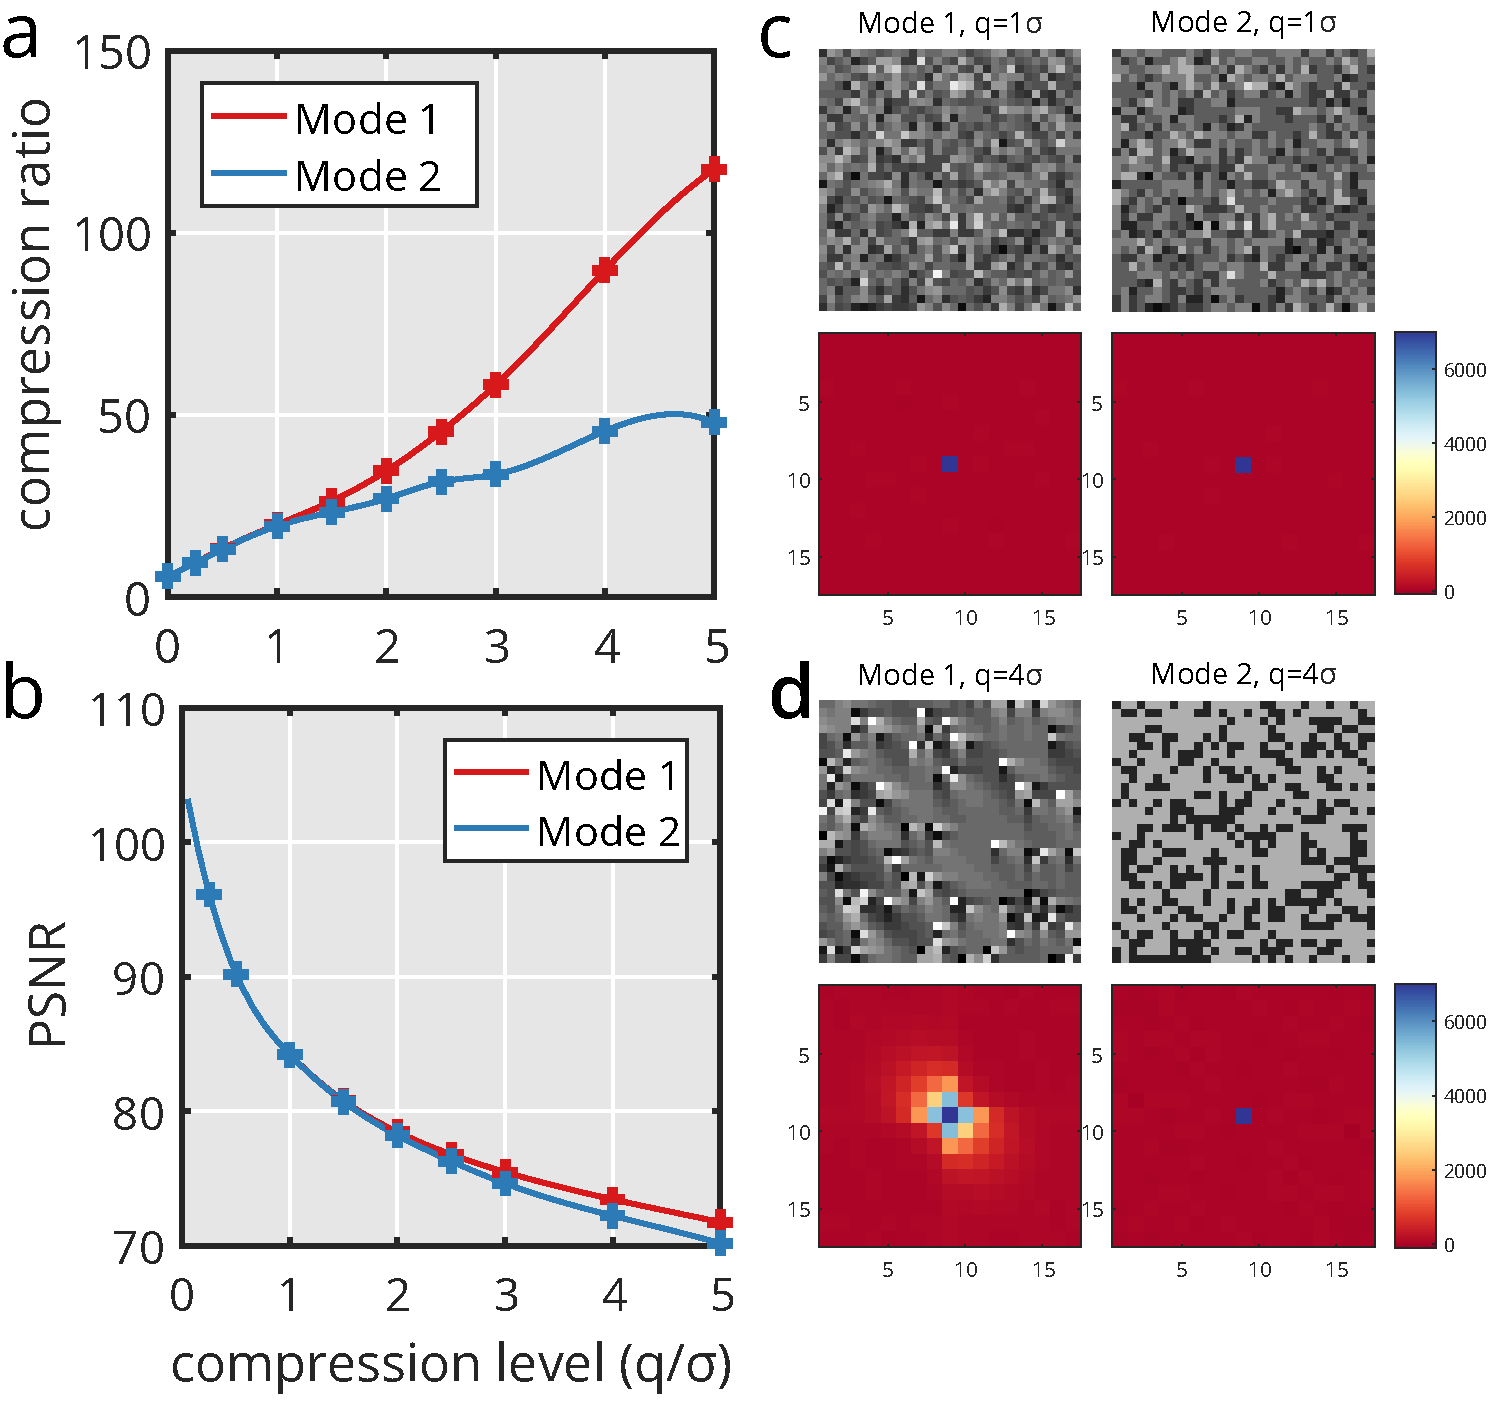
\includegraphics[page=1,width=0.6\textwidth]{swapping}
      \bcaption[Options for noise-dependent lossy compression]{Comparing Mode 1 (prediction then quantization) and Mode 2 (quantization then prediction) of noise-dependent lossy compression in terms of compression ratio, peak signal-to-noise ratio (PSNR) and spatial correlations introduced to random noise. (\textbf{a}) Compression ratio as a function of the quantization step for Mode 1 and Mode 2. (\textbf{b}) PSNR as a function of the quantization step for Mode 1 and Mode 2. (\textbf{c, d}) Random noise was compressed at various quantization steps both for Mode 1 and Mode 2. Autocorrelation was calculated for the compressed images to see whether the compression introduces any spatial correlation between the pixels. For q=1$\upsigma$ both modes are free of correlation (\textbf{c}, top: compressed images, bottom: autocorrelation), however, for q=4$\upsigma$ Mode 1 exhibits a correlation pattern (\textbf{d}, top left: compressed image, bottom left: autocorrelation) that is not present in Mode 2 (\textbf{d}, top right compressed image, bottom right: autocorrelation). For more discussion, see \autoref{sec:wnl}.}
      \label{fig:swapping}
    \end{figure}


    \subsubsection{Additional noise introduced by compression}
    \label{sec:extraNoise}

    When applying quantization to any kind of data, the quantization error can be modeled as an additional uniform noise with standard deviation of $\frac{\delta}{\sqrt{12}}$, where $\delta$ is the quantization step size \cite{gray_quantization_1998}. During compression the quantization is proportional to the standard deviation of the original image noise, thus the noise on the decompressed image will be:
    \begin{equation}
      \sigma_{out} = \sigma_{in} \cdot \sqrt{1+ \frac{q^2}{12}}
    \end{equation}
    For the WNL case, when $q = 1 \sigma$ this means an increase of 4\%, which also coincides with the measured increase of localization error for single molecule localization (\autoref{fig:wnlSMLM}a). However, this is not the only source of additional noise we have to consider, because at the decompression step there is a possibility of getting floating point results after applying the inverse of the compression steps, and for most applications these have to be coerced to integer numbers. This effectively adds a second quantization, but now at a constant quantization step of 1. This results in an additional uniform noise with variance of $\frac{1}{12}$:
    \begin{equation}
      \sigma_{out} = \sigma_{in} \cdot \sqrt{1+ \frac{q^2}{12}} + \frac{1}{12}
      \label{eq:extraNoise}
    \end{equation}
    We verified this by compressing 512 images (1024\texttimes 1024 pixels) of random Poisson noise with different means (1--512), and calculated the standard deviation for each frame after the decompression step. Finally, we plotted the ratio $\sigma_{out}/\sigma_{in}$ as a function of the mean $m$ (\autoref{fig:extraNoise}), and we found that it is in very good agreement with the theory outlined above.

    

    

    \begin{figure}
      \centering
      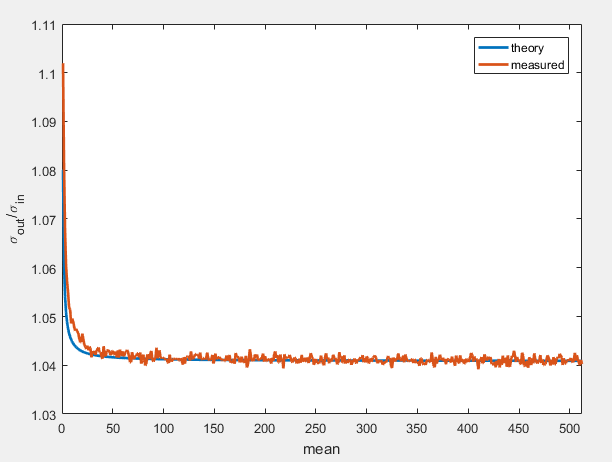
\includegraphics[width=0.5\textwidth]{extraNoise}
      \bcaption[Theoretical and measured increase in image noise for WNL compression]{Validating \autoref{eq:extraNoise}, we plot the relative increase in image noise as a function of the mean. Blue line: plot of \autoref{eq:extraNoise} Red line: plot of measured data. To obtain the measurement, we compressed a stack of 512 images consisting of Poisson noise, each with a different mean. After WNL compression the dataset was read in Matlab, and the standard deviation was calculated for each frame. The ratio $\sigma_{in}/\sigma_{out}$ is plotted as a function of the mean.}
      \label{fig:extraNoise}
    \end{figure}

  \subsection{Evaluation of the compression algorithm}
    \label{sec:evalB3D}
  We compared our algorithm’s performance with some of the most commonly used image formats in the scientific field: TIFF (LZW) and JPEG2000. Furthermore, we also included the state of the art KLB compression \cite{amat_efficient_2015}, which was especially designed for fast compression of large light-sheet datasets. We measured compression speed, decompression speed and resulting file size for all algorithms (\autoref{fig:bubbles}a). Only \b3d is capable of handling the sustained high data rate of modern sCMOS cameras typically used in light-sheet microscopy, while still maintaining compression ratios comparable to more complex, but much slower algorithms (\autoref{tab:performance} in Appendix \ref{app:tables}).

  % "TODO" We define the mode where the quantization step is equal to the noise (q=1σ) as within-noise-level (WNL) compression.
  Using the noise-dependent lossy mode with $q=1\sigma$ (WNL), the compression ratio massively increases for all imaging modalities compared to the lossless mode (\autoref{fig:bubbles}b) without any apparent loss in image quality (\autoref{fig:wnlSamples}). Furthermore, the average compression error is considerably smaller than the image noise itself (\autoref{fig:RMSD}).

    \begin{figure}[tpb]
      \centering
      \begin{subfigure}{0.49\textwidth}
        \centering
        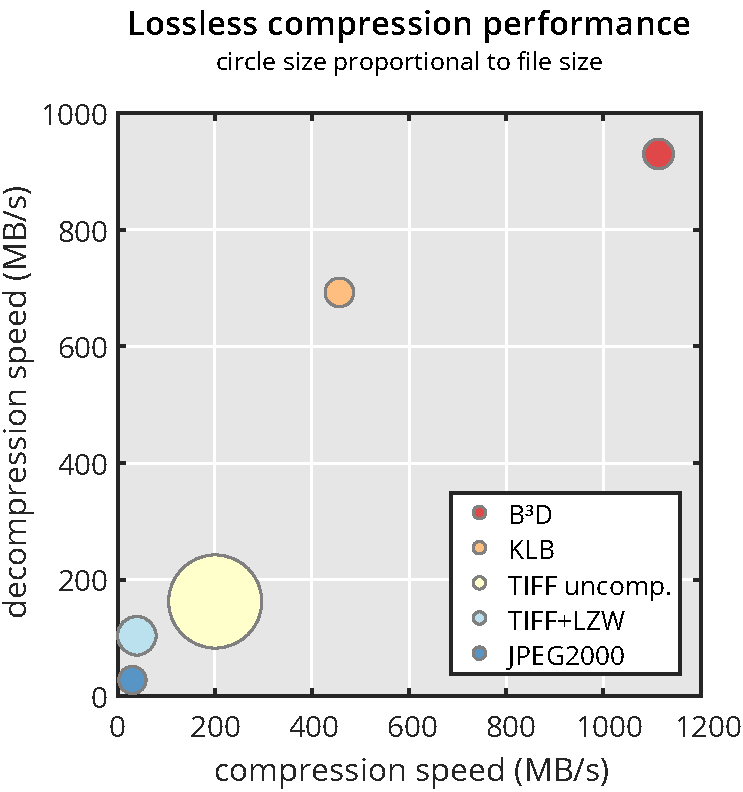
\includegraphics[page=1,height=0.9\textwidth]{bubbles}
        \caption{}
      \end{subfigure}      
      \begin{subfigure}{0.49\textwidth}
        \centering
        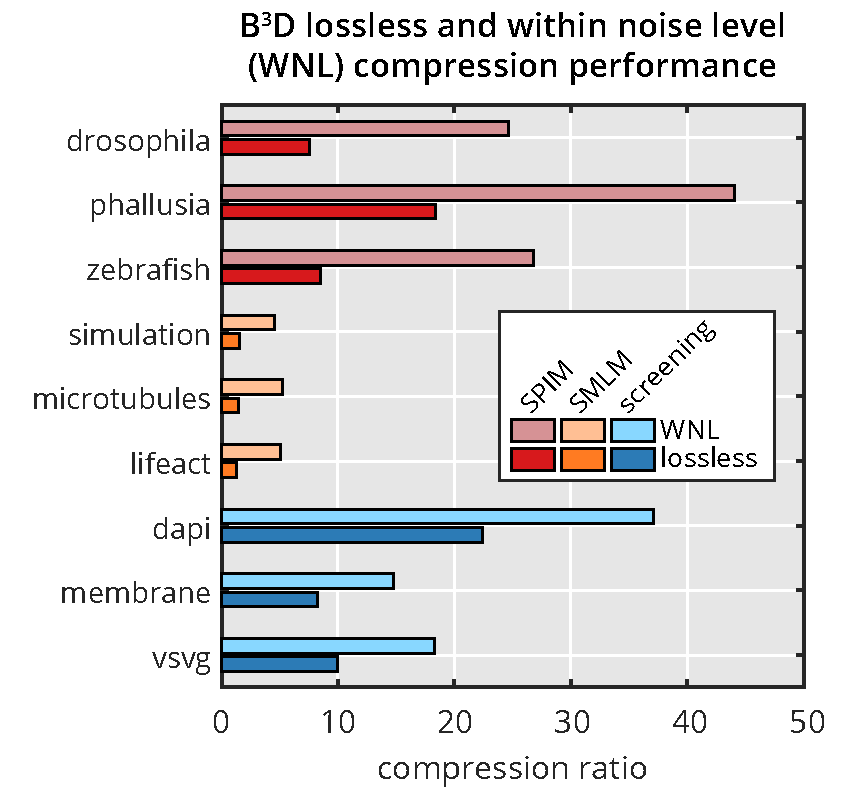
\includegraphics[page=1,height=0.9\textwidth]{Fig1c_compressionBars}
        \caption{}
      \end{subfigure}      
      \bcaption[Compression performance]{(\textbf{a}) Performance comparison of our \b3d compression algorithm (red circle) vs. KLB (orange), uncompressed TIFF (light yellow), LZW compressed TIFF (light blue) and JPEG2000 (blue) regarding write speed (horizontal axis), read speed (vertical axis) and file size (circle size). (see also Table \ref{tab:performance}). (\textbf{b}) WNL compression performance compared with lossless performance for 9 different dataset representing 3 imaging modalities (SPIM, SMLM, screening). Compression ratio = original size / compressed size. For description of datasets see Table \ref{tab:datasets} in Appendix B.}
      \label{fig:bubbles}
    \end{figure}

    % \begin{figure}[tpb]
    %   \centering
    %   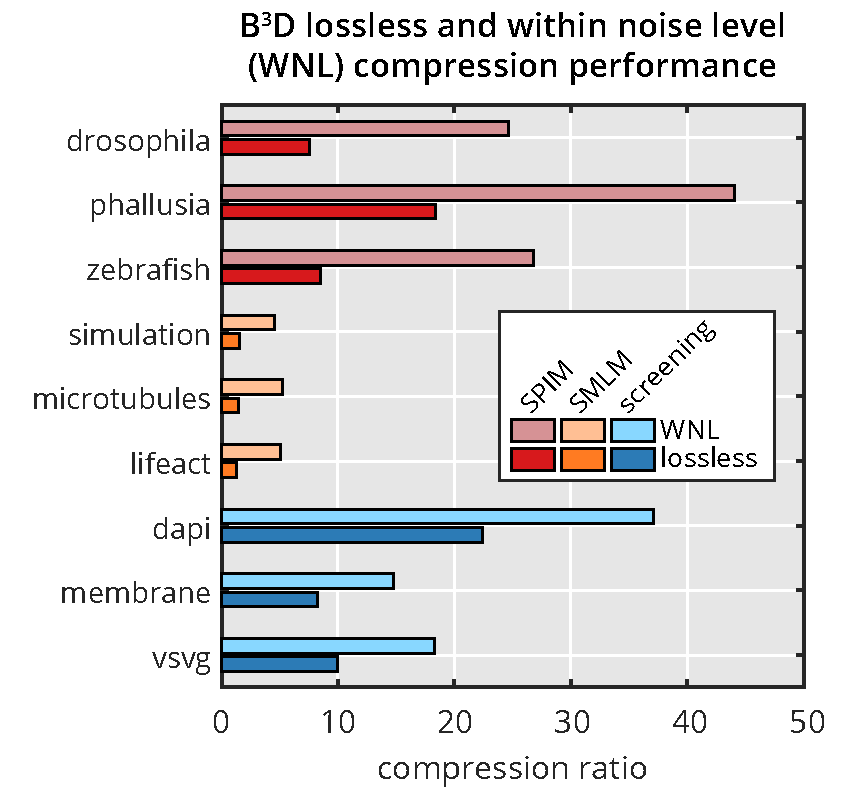
\includegraphics[page=1,height=0.4\textwidth]{Fig1c_compressionBars}
    %   \bcaption[within-noise-level compression performance]{WNL compression performance compared with lossless performance for 9 different dataset representing 3 imaging modalities (SPIM, SMLM, screening). Compression ratio = original size / compressed size. For description of datasets see Table \ref{tab:datasets} in Appendix B.}
    %   \label{fig:benchmark}
    % \end{figure}



    \begin{figure}[tpb]
      \centering
      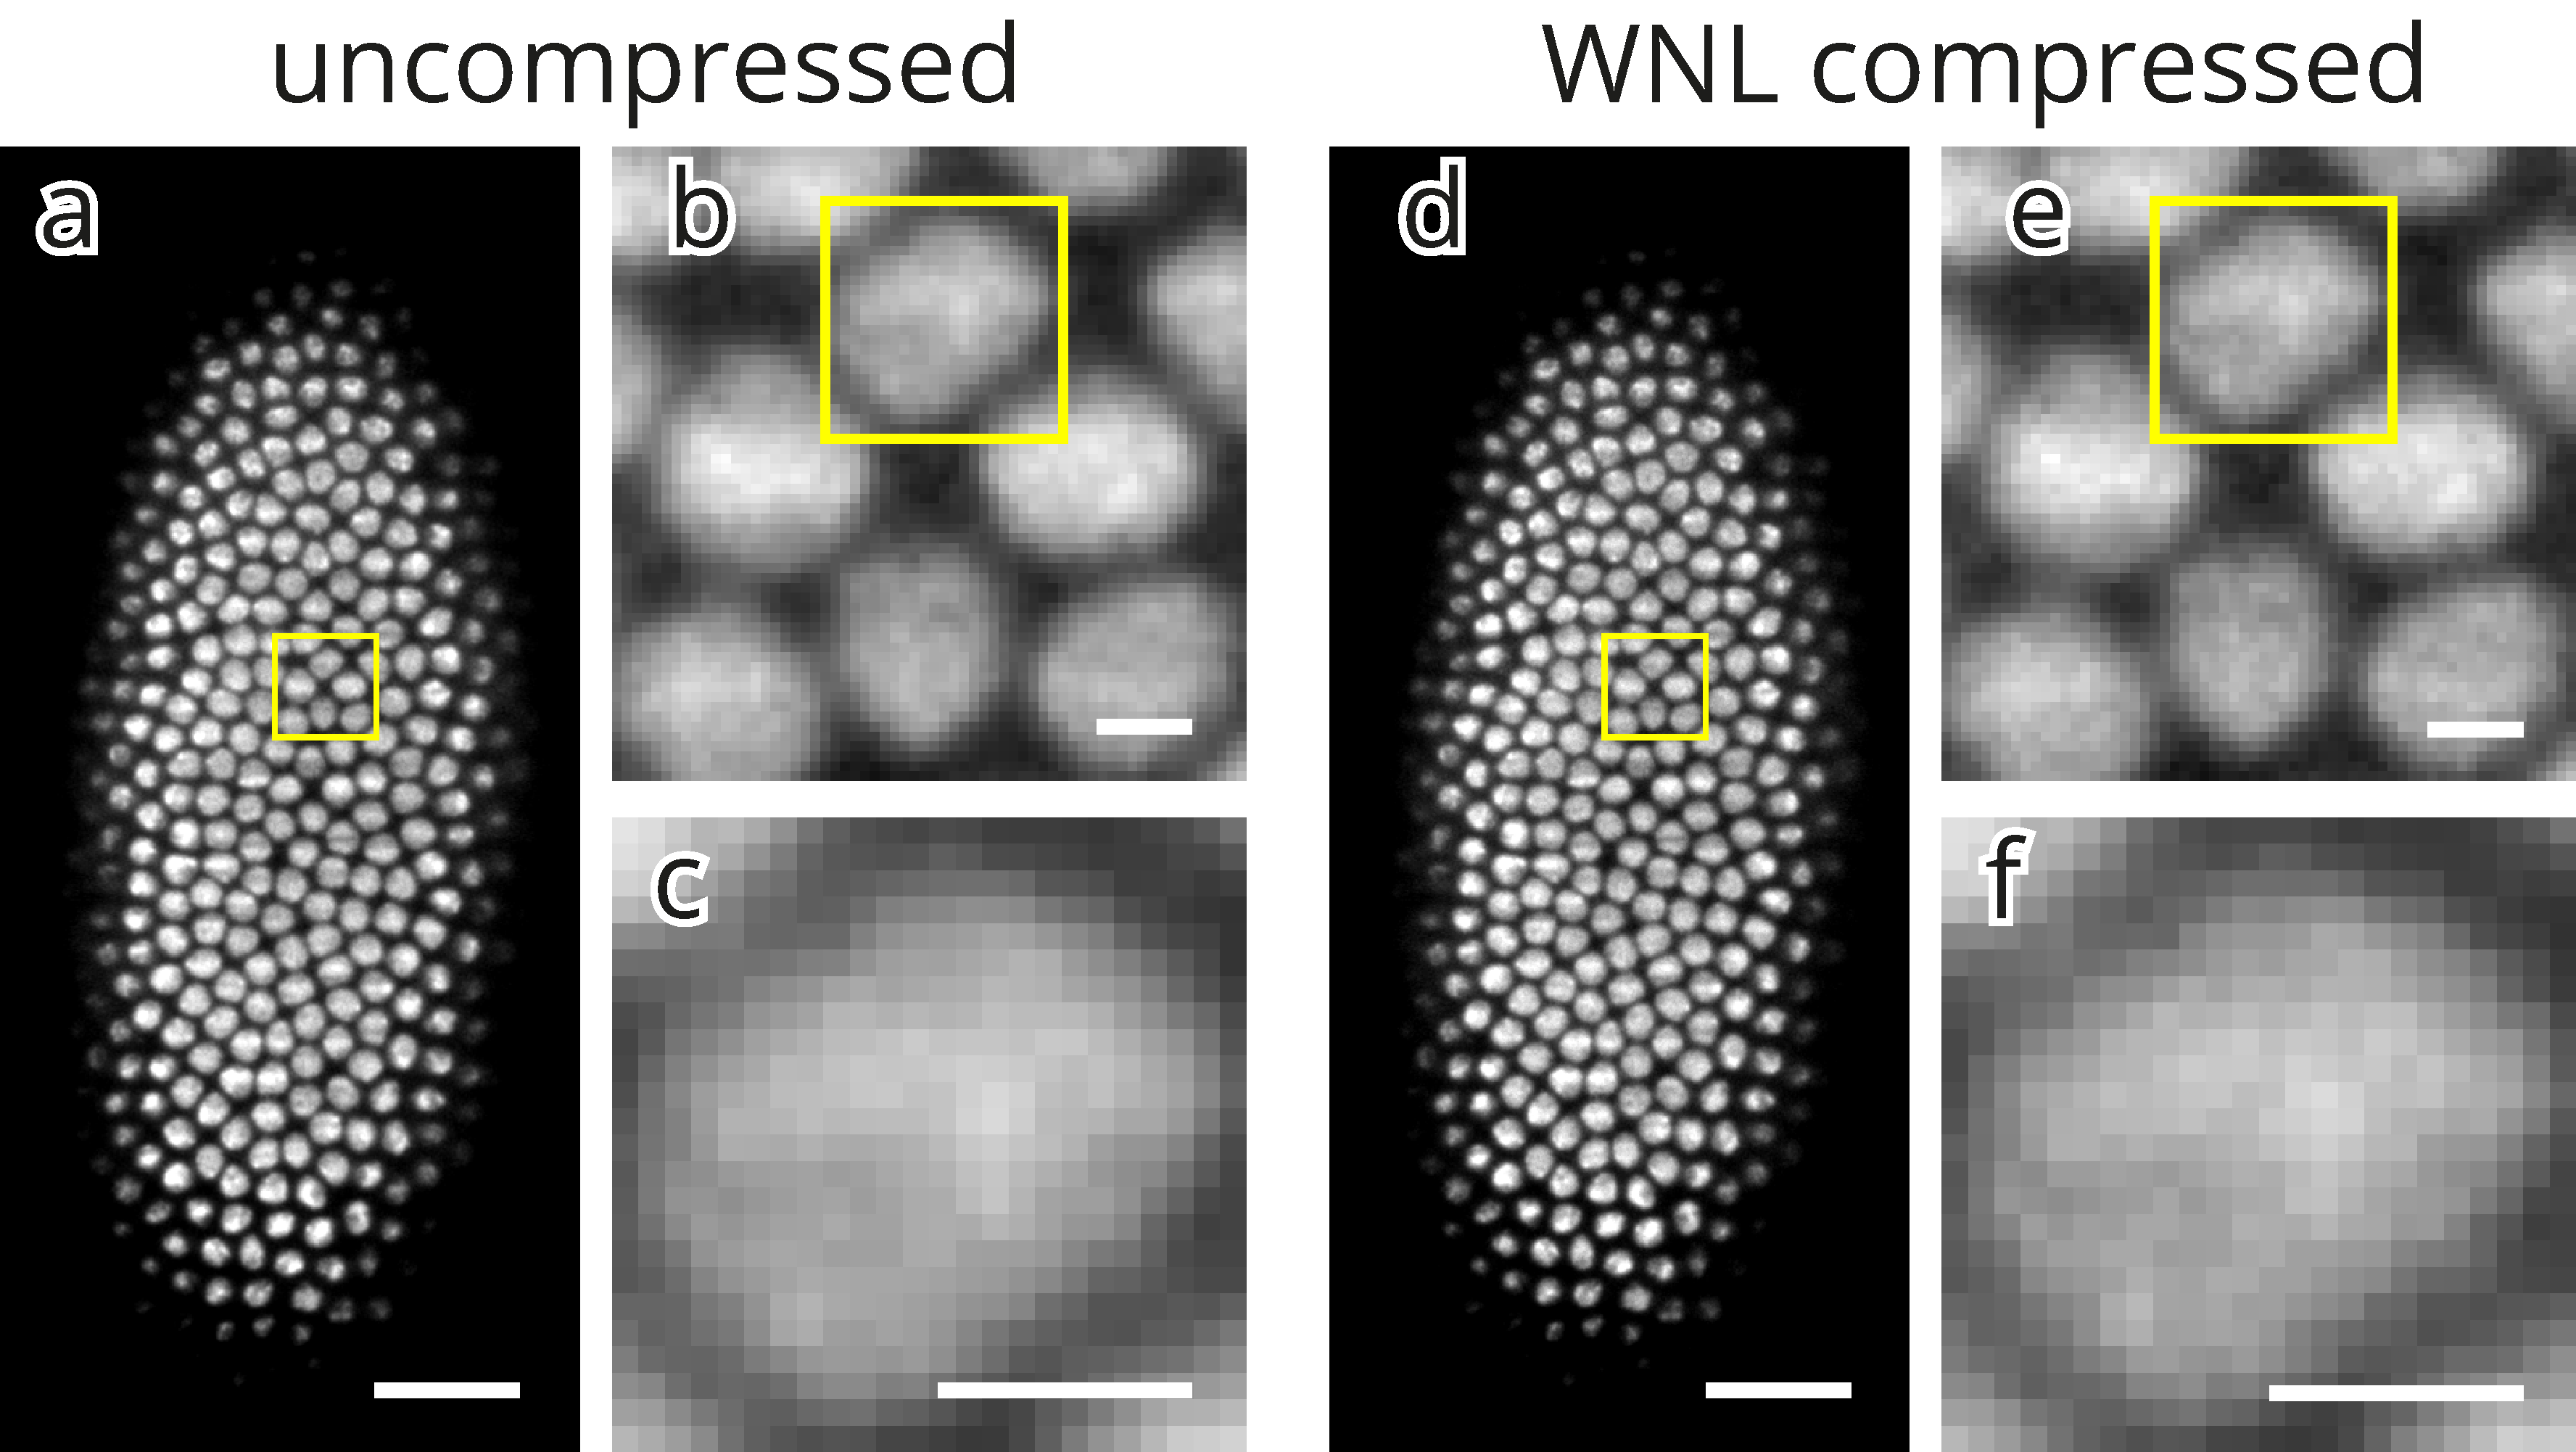
\includegraphics[page=1,width=0.7\textwidth]{wnlSamples}
      \bcaption[Image quality of a WNL compressed dataset]{WNL compression of a \textit{Drosophila} recording taken in the MuVi-SPIM setup. Compression ratio: 19.83. (a–c) Uncompressed image of the whole field of view (a), and zoomed in smaller regions (b, c). (d–f) WNL compressed image of the whole field of view (d), and zoomed in smaller regions (e, f). Scale bars: \SI{25}{\micro m} (a, e); \SI{2.5}{\micro m} (b, c, e, f).}
      \label{fig:wnlSamples}
    \end{figure}

    \begin{figure}[tpb]
      \centering
      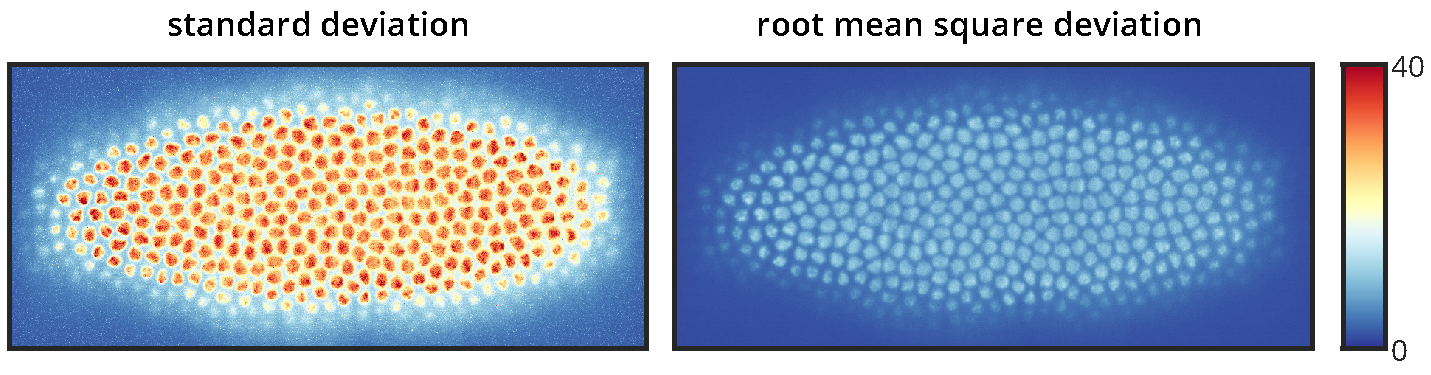
\includegraphics[page=1,width=1\textwidth]{SFig4_RMSDvsSD_rotated}
      \bcaption[Compression error compared to image noise]{To compare the difference arising from WNL compression to image noise, we imaged a single plane 100 times in a \textit{Drosophila melanogaster} embryo expressing H2Av-mCherry nuclear marker at \SI{38}{ms} intervals. The whole acquisition took \SI{3.8}{s}, for which the sample can be considered stationary. To visualize image noise, the standard deviation was calculated for the uncompressed images (left). All images were then WNL compressed, and the root mean square deviation was calculated compared to the uncompressed images (right). The root mean square deviation on average is 3.18 times smaller than the standard deviation of the uncompressed images.}
      \label{fig:RMSD}
    \end{figure}

    To see how the noise-dependent compression affects common imaging pipelines, we tested the effect of different levels of compression on 3D nucleus and membrane segmentation in light-sheet microscopy, and on single-molecule localization accuracy in superresolution microscopy.
    First, we imaged a \textit{Drosophila melanogaster} embryo expressing an H2Av-mCherry nuclear marker in the MuVi-SPIM and segmented the nuclei with Ilastik \cite{sommer_ilastik:_2011} (\autoref{fig:wnlDroso}a and \autoref{sec:methodsB3D}). Then we performed noise dependent compression at various quality levels and calculated the segmentation overlap compared to the uncompressed stack (\autoref{sec:methodsB3D}). At WNL compression ($q=1 \sigma$) the segmentation overlap is almost perfect (\autoref{fig:wnlDroso}b) with an overlap score of 0.996. Even when increasing the quantization step to $4\sigma$ (\autoref{fig:wnlDroso}c) the overlap score stays at 0.98 and only drops below 0.97 when the compression ratio is already above 120 (quantization step of $5\sigma$, \autoref{fig:wnlDroso}d).
    We got similar results for a membrane segmentation pipeline that is used with \textit{Phallusia mammillata} embryos (\autoref{fig:wnlPhallusia}and \autoref{sec:methodsB3D}).

    \begin{figure}[tpb]
      \centering
      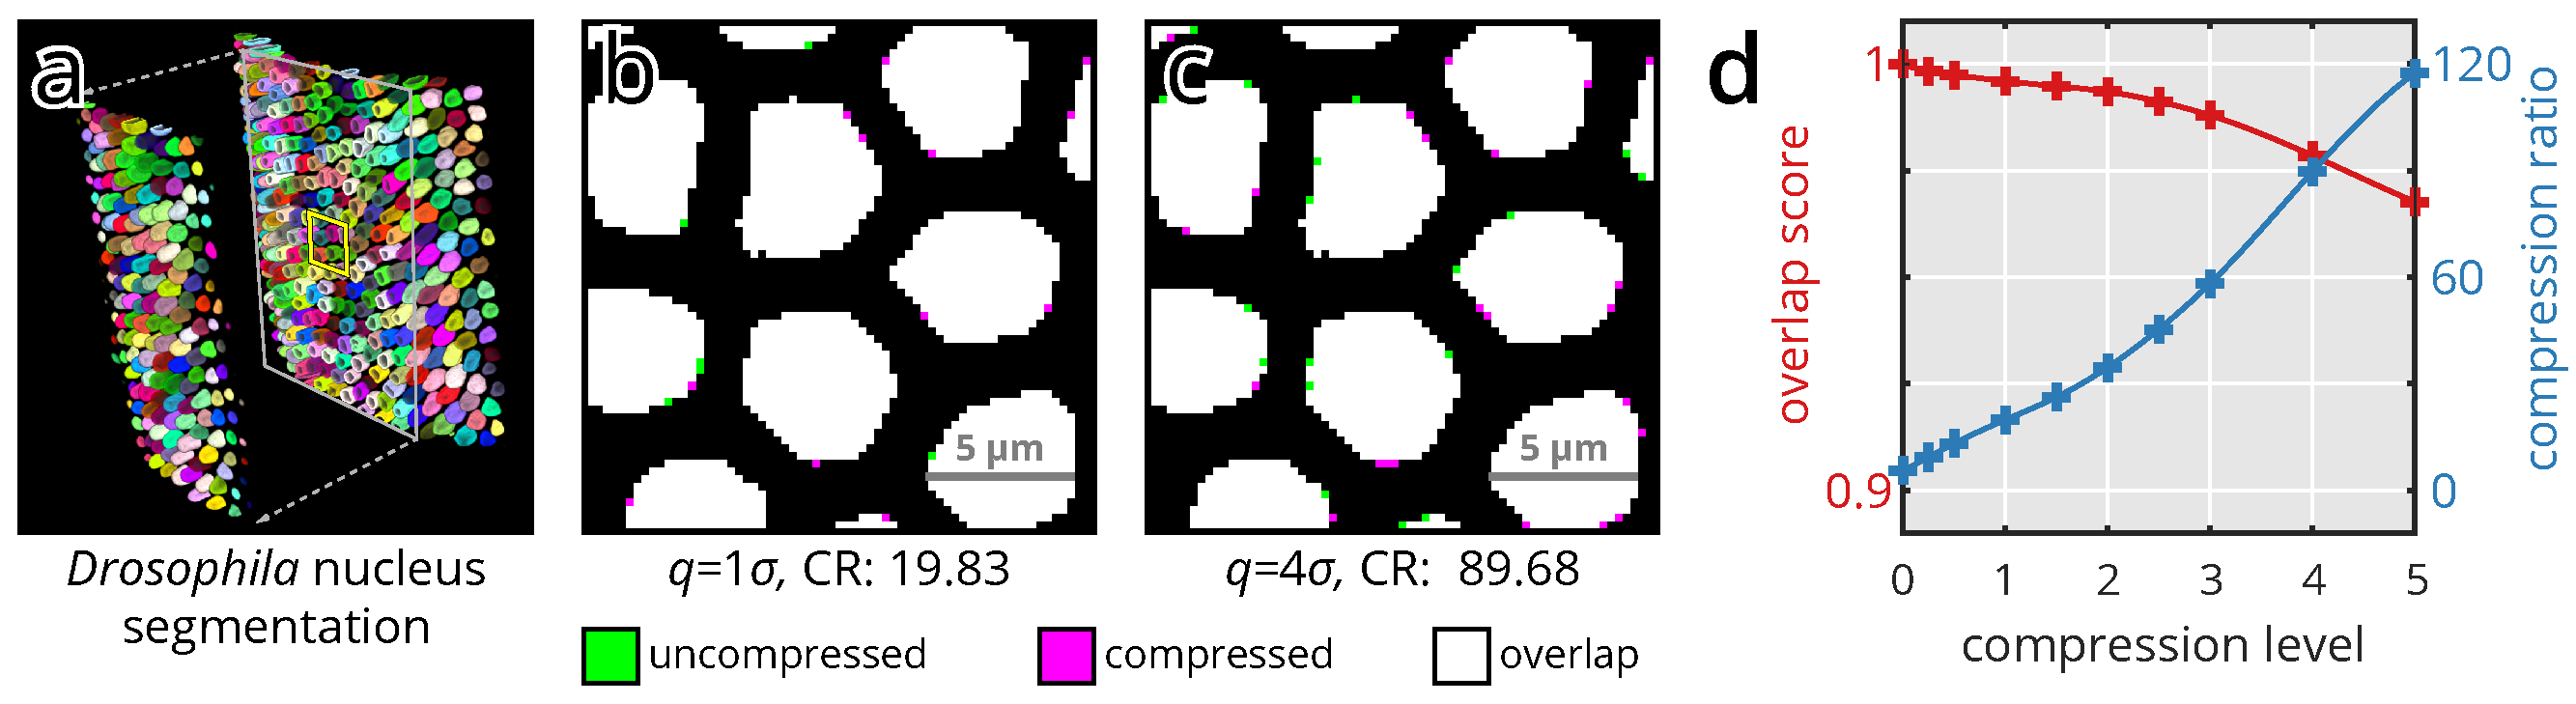
\includegraphics[page=1,width=1\textwidth]{LLvsB3D}
      \bcaption[Influence of noise-dependent lossy compression on 3D nucleus segmentation]{A \textit{Drosophila melanogaster} embryo expressing H2Av-mCherry nuclear marker was imaged in MuVi-SPIM \cite{krzic_multiview_2012}, and 3D nucleus segmentation was performed (\autoref{sec:methodsB3D}) (\textbf{a}). The raw dataset was subsequently compressed at increasingly higher compression levels, and segmented based on the training of the uncompressed data. To visualize segmentation mismatch, the results of the uncompressed (green) and compressed (magenta) datasets are overlaid in a single image (\textbf{b}, \textbf{c}; overlap in white). Representative compression levels were chosen at two different multiples of the photon shot noise, at q=1$\upsigma$ (\textbf{b}) and q=4$\upsigma$ (\textbf{c}). For all compression levels the segmentation overlap score (\autoref{sec:methodsB3D}) was calculated and is plotted in (\textbf{d}) along with the achieved compression ratios.}
      \label{fig:wnlDroso}
    \end{figure}

    \begin{figure}[tpb]
      \centering
      \includegraphics[page=3,width=1\textwidth]{LLvsB3D}
      \bcaption[Influence of noise-dependent lossy compression on 3D membrane segmentation]{A \textit{Phallusia mammillata} embryo expressing PH-citrine membrane marker was imaged in MuVi-SPIM \cite{krzic_multiview_2012}, and 3D membrane segmentation was performed (\autoref{sec:methodsB3D}) (\textbf{a}). The raw dataset was subsequently compressed at increasingly higher compression levels, and segmented using the same settings as the uncompressed data. To visualize segmentation mismatch, the results of the uncompressed (green) and compressed (magenta) datasets are overlaid in a single image (\textbf{b, c}; overlap in white). Representative compression levels were chosen at two different multiples of the photon shot noise, at q=1.6$\upsigma$ (\textbf{b}) and q=4.8$\upsigma$ (\textbf{c}). For all compression levels the segmentation overlap score (\autoref{sec:methodsB3D}) was calculated and is plotted in (\textbf{d}) along with the achieved compression ratios.}
      \label{fig:wnlPhallusia}
    \end{figure}

    Next, we evaluated our compression algorithm in the context of single molecule localization microscopy (SMLM), and measured how the localization precision is affected when compressing the raw images by an increasing compression ratio. We compressed an SMLM dataset of immuno-detected microtubules (\autoref{fig:wnlSMLM}a) with increasing compression levels. For WNL compression ($q=1\sigma$) no deterioration of the image was visible (\autoref{fig:wnlSMLM}b), and even for the case of $q=4\sigma$ the compression induced errors were much smaller than the resolvable features (\autoref{fig:wnlSMLM}c). To quantify the impact of compression on the localization error, we used a simulated dataset (\autoref{sec:methodsB3D}) and compared the localization output of different compression levels to the ground truth (\autoref{fig:wnlSMLM}d). Lossless compression resulted in a compression ratio of 2.7, whereas WNL compression reached a compression ratio of 5.0, while increasing the localization error by only 4\%. This also coincides with the theoretical increase of image noise (\autoref{sec:extraNoise}). Furthermore, the increase in localization error was not dependent on the signal to background noise ratio (\autoref{fig:SFig6_locprecVsNphotons}).

    \begin{figure}[tpb]
      \centering
      \includegraphics[page=2,width=1\textwidth]{LLvsB3D}
      \bcaption[Influence of noise-dependent lossy compression on single-molecule localization]{Microtubules, immunolabeled with Alexa Fluor 647 were imaged by SMLM (\textbf{a}). The raw dataset was compressed at increasingly higher compression levels, and localized using the same settings as the uncompressed data. To visualize localization mismatch, the results of the uncompressed (green) and compressed (magenta) datasets are overlaid in a single image (\textbf{b}, \textbf{c}; overlap in white). Two representative compression levels were chosen at q=1$\upsigma$ (\textbf{b}) and q=4$\upsigma$ (\textbf{c}). To assess the effects of compression on localization precision, a simulated dataset with known emitter positions was compressed at various levels. For all compression levels the relative localization error (normalized to the Cramér–Rao lower bound) was calculated and is plotted in (\textbf{d}) along with the achieved compression factors.}
      \label{fig:wnlSMLM}
    \end{figure}

    \begin{figure}[tpb]
      \centering
      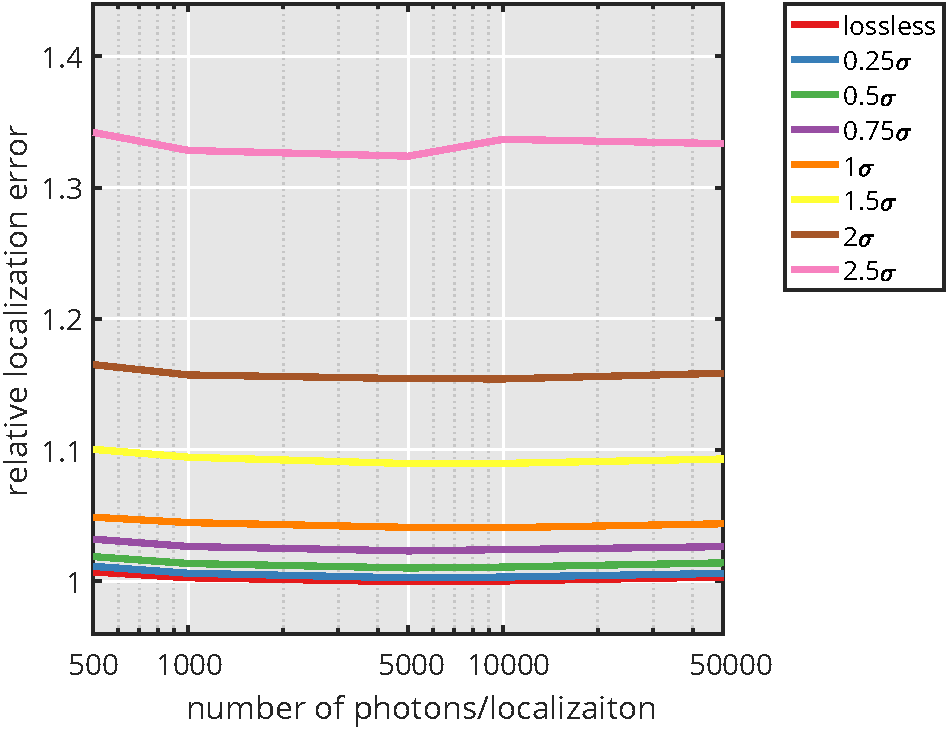
\includegraphics[page=1,width=0.5\textwidth]{SFig6_locprecVsNphotons}
      \bcaption[Change in localization error only depends on selected quantization step]{We simulated multiple datasets (\autoref{sec:methodsB3D}) with different average photon numbers per localization. Background was kept at a constant average of 20 photons/pixel. Datasets were compressed at multiple compression levels (see legend), and localization error relative to the Cramér-Rao lower bound was calculated. The relative localization error only depends on the compression level, and not on the signal to background illumination ratio.}
      \label{fig:SFig6_locprecVsNphotons}
    \end{figure}



  
  % Anscombe \cite{anscombe_transformation_1948}
  % optimal inverse Anscombe \cite{makitalo_optimal_2011,makitalo_closed-form_2011}
  % optimal inverse generalized Anscombe \cite{makitalo_optimal_2013}

  \subsection{HDF5 integration}
  To make our compression method more accessible, we developed a filter plugin for HDF5. Because of its versatility, HDF5 has emerged as the \textit{de facto} standard in the open source light-sheet microscopy field, and is also the basis for the widely used BigDataViewer \cite{pietzsch_bigdataviewer:_2015} in Fiji \cite{schindelin_fiji:_2012}. Starting from version 1.8.11 (May 2013), HDF5 supports dynamically loaded filters, and is able to load third party components without having to modify any already installed files. When loading a \b3d compressed image in an HDF5 enabled application, the library automatically calls our filter plugin, decompresses the image on the GPU, and copies it back into CPU memory.
  
  Since HDF5 is extensively used in many scientific/image analysis software, this plugin format is especially suitable to equip existing software with compression/decompression capabilities. To read compressed files no modification is required, and any software supporting HDF5 should be compatible. The following software have been tested with our filter plugin and are able to read \b3d compressed files:
  Fiji (also with BigDataViewer), Imaris 8.4.1, Ilastik 1.2.0, Matlab R2016a, Python 2.7.10 and 3.5.3, LabVIEW 2015, C++.
  
  Writing compressed HDF5 files is possible if the user has direct control over the file writing routine, as an additional command is required to set up compression. This functionality has been tested in the following environments: C++, Python 2.7.10 and 3.5.3, LabVIEW 2015.


  %#     ## ######## ######## ##     ## 
  %##   ### ##          ##    ##     ## 
  %### #### ##          ##    ##     ## 
  %# ### ## ######      ##    ######### 
  %#     ## ##          ##    ##     ## 
  %#     ## ##          ##    ##     ## 
  %#     ## ########    ##    ##     ## 

\subsection{Methods}
  \label{sec:methodsB3D}
\subsubsection{Compression benchmarking}
For all presented benchmarks, TIFF and JPEG2000 performance was measured through MATLAB's imwrite and imread functions, while KLB and \b3d performance was measured in C++. All benchmarks were run on a computer featuring 32 processing cores (2×Intel Xeon E5-2620 v4), \SI{128}{GB} RAM and an NVIDIA GeForce GTX 970 graphics processing unit. Read and write measurements were performed in RAM to minimize I/O overhead, and are an average of 5 runs. SMLM datasets were provided by Joran Deschamps (EMBL, Heidelberg), and were originally published in \cite{deschamps_3d_2014} and \cite{deschamps_efficient_2016}. Screening datasets were provided by Jean-Karim Hériché (EMBL, Heidelberg), and were originally published in \cite{simpson_genome-wide_2012}

\subsubsection{Light-sheet imaging}
\textit{Drosophila} embryos were imaged in the MuVi-SPIM setup \cite{krzic_multiview_2012} using the electronic confocal slit detection (eCSD) \cite{de_medeiros_confocal_2015}. Embryos were collected on an agar juice plate, and dechorionated in 50\% bleach solution for \SI{1}{min}. The embryos were then mounted in a shortened glass capillary (Brand \SI{100}{\micro l}) filled with 0.8\% GelRite (Sigma-Aldrich), and pushed out of the capillary to be supported only by the gel.

\subsubsection{3D nucleus segmentation}
3D nucleus segmentation of \textit{Drosophila} embryos was performed using Ilastik \cite{sommer_ilastik:_2011}. The original dataset was compressed at different quantization levels, then upscaled in z to obtain isotropic resolution. To identify the nuclei, we used the pixel classification workflow, and trained it on the uncompressed dataset. This training was then used to segment the compressed datasets as well. Segmentation overlap was calculated in Matlab using the Sørensen–Dice index \cite{sorensen_method_1948,dice_measures_1945}:
\begin{equation}
  QS = 2 \left| A \cap B \right| / \left( |A| + |B| \right)
\end{equation}
where the sets $A$ and $B$ represent the pixels included in two different segmentations.

\subsubsection{3D membrane segmentation}
Raw MuVi-SPIM recordings of \textit{Phallusia mammillata} embryos expressing PH-citrine membrane marker were kindly provided by Ulla-Maj Fiuza (EMBL, Heidelberg). Each recording consisted of 4 views at 90 degree rotations. The views were fused using an image based registration algorithm followed by a sigmoidal blending of the 4 views.
% The fusion software was developed by Leo Guignard (Janelia Research Campus, Ashburn, Virginia).
The fused stack was then segmented using the MARS algorithm \cite{fernandez_imaging_2010} with an hmin parameter of 10. The raw data (all 4 views) was compressed at different levels, and segmented using the same pipeline. Segmentation results were then processed in Matlab to calculate the overlap score for the membranes using the Sørensen–Dice index.

\subsubsection{Single-molecule localization imaging}
In order to visualize microtubules, U2OS cells were treated as in \cite{deschamps_3d_2014} and imaged in a dSTORM buffer \cite{heilemann_subdiffraction-resolution_2008}. In brief, the cells were permeabilized and fixed with glutaraldehyde, washed, then incubated with primary tubulin antibodies and finally stained with Alexa Fluor 647 coupled secondary antibodies. The images were recorded on a home-built microscope previously described \cite{deschamps_3d_2014}, in its 2D single-channel mode.

\subsubsection{Single-molecule localization data analysis}
Analysis of single-molecule localization data was performed on a custom-written MATLAB software as in \cite{deschamps_efficient_2016}. Pixel values were converted to photon counts according to measured offset and calibrated gain of the camera (EMCCD iXon, Andor). The background was estimated with a wavelet filter \cite{izeddin_wavelet_2012}, background-subtracted images were thresholded and local maxima were detected on the same images. 7-pixel ROIs around the detected local maxima were extracted from the raw images and fitted with a GPU based MLE fitter \cite{smith_fast_2010}. Drift correction was performed based on cross-correlation. Finally, images were
reconstructed by filtering out localizations with a high uncertainty (>\SI{30}{nm}) and large PSF (>\SI{150}{nm}) and Gaussian rendering.

\subsubsection{Simulation of single-molecule localization data}
Single molecule localization datasets were simulated in Matlab by generating a grid of pixelated Gaussian spots with standard deviation of 1 pixel. With a pixel size of a 100 nm, this corresponds to a FWHM of 235.48 nm. The center of each spot was slightly offset from the pixel grid at 0.1 pixel increments in both x and y directions. To this ground truth image a constant value was added to simulate illumination background, and finally Poisson noise was applied to the image. This process was repeated 10,000 times to obtain enough images for adequate accuracy.

\subsubsection{Code availability}
Code used for analyzing data, \b3d source code and compiled binaries, including a filter plugin for HDF5, are available for download at \url{https://git.embl.de/balazs/B3D}.






\section{Discussion}

In this chapter we presented a real-time image preprocessing and compression pipeline for multiview light-sheet microscopy. This pipeline is capable of fusing 

Our algorithm is implemented in C++, and allows for easy integration through an API with various programming languages. The library was tested on Linux (Ubuntu 16.04) and Windows (10). Additionally, we implemented a filter plugin for HDF5 which enables a seamless integration in all software packages that are supporting the native HDF5 library, such as Matlab, Python, Imaris, or Ilastik. Due to \b3d’s efficient compression ratio and its high decompression speed, loading data is often accelerated: For a state-of-the-art hard drive with \SI{200}{MB/s} bandwidth, loading a \SI{2}{GB} uncompressed 3D stack of images takes about 10 seconds. With an average compression ratio of 20 fold in the WNL mode, the loading time is reduced to 0.5 seconds followed by 2 seconds of decompression, which yields a factor of four speed-up.

It is also worth to note, that the achieved WNL compression reduces the camera data rate to below \SI{40}{MB/s}, well below the \SI{1}{Gb/s} Ethernet standard. This enables to use current network infrastructure to move data to long term storage and even makes the use of cloud services possible. Altogether, \b3d, our efficient GPU-based image compression library allows for exceptionally fast compression speed and greatly increases compression ratio with its WNL scheme, offering a versatile tool that can be easily tailored to any high-speed microscopy environment.